\documentclass[11pt]{article}
\usepackage[utf8]{inputenc}
\usepackage[spanish,es-tabla,es-nodecimaldot]{babel}

% Paquetess

\usepackage{amsmath}
\usepackage{amsthm}
\usepackage{amsfonts}
\usepackage{amssymb}
\usepackage{makeidx}
\usepackage{graphicx}
\usepackage{lmodern}
\usepackage[dvipsnames]{xcolor} 
\usepackage{fancyhdr}
\usepackage{geometry}
\usepackage{lastpage}		
\usepackage{array}			 % Para fjar tamaño de columnas
\usepackage{tikz}
\usepackage{subcaption}
\usepackage{caption}
\usepackage{pgfplots} % Para controlar la perspectiva
\RequirePackage{siunitx}
\usepackage{extramarks} % Para poder usar firstleftmarks
\usepackage[version=4]{mhchem} % Para poder usar formulas de reacciones nucleares
\usepackage{chemfig}
\usepackage{xcolor}
\RequirePackage[most]{tcolorbox}
\usepackage{enumitem}
\usepackage{physics}
%\usepackage{background}
\usepackage{eso-pic} % Para insertar imágenes de fondo específicas
\usepackage[absolute,overlay]{textpos} % Paquete para colocar elementos en posiciones absolutas
\usepackage{wrapfig}
\usepackage{booktabs}
\usepackage{float} % en el preámbulo

\setlength{\parindent}{0pt} % Elimina la sangría
\newtcolorbox{mybox}{colback=black!5!white,
	colframe=black!75!black}

\newtcolorbox{Anotacion}{colback=red!5!white,
	colframe=red!75!red}


%##############################################################################
%######### Ponemos el decimal con . ###########################################
%##############################################################################

\sisetup{output-decimal-marker={.},
	% exponentes ------------------------
	exponent-mode=threshold,
	exponent-thresholds=-3:3, % non usar exponentes 10^{-2,-1, 0, 1,2}
	% redondear -------------------------
	% round-mode=figures, % cifras sig
	% round-mode=places, % cantos decimales
	round-mode=uncertainty, % cifras sig da incerteza (necesario usar erro)
	round-precision=2,
	uncertainty-mode = separate,
	print-unity-mantissa=false,
	% unidades --------------------------
	inter-unit-product = \ensuremath{{}\cdot{}}, % separacion entre unidades
	% per-mode=power-positive-first, % so furrula con metodo interpretado puro
	inline-per-mode=single-symbol,
	display-per-mode=fraction,
}

%##############################################################################
%######### Para codigo python #################################################
%##############################################################################

\definecolor{codegreen}{rgb}{0,0.6,0}
\definecolor{codegray}{rgb}{0.5,0.5,0.5}
\definecolor{codepurple}{rgb}{0.58,0,0.82}

\usepackage{listings}


%\lstdefinestyle{mystyle}{	backgroundcolor=\color{backcolour},   	commentstyle=\color{codegreen},	keywordstyle=\color{magenta},	numberstyle=\tiny\color{codegray},	stringstyle=\color{codepurple},	basicstyle=\ttfamily\footnotesize,	breakatwhitespace=false,         	breaklines=true,                 	captionpos=b,                    	keepspaces=true,                 	numbers=left,                    	numbersep=5pt,                  	showspaces=false,                	showstringspaces=false,	showtabs=false,                  	tabsize=2}

%\lstset{style=mystyle}
%\usepackage{background}     % Para manejar el fondo

%%%%%%%%%%%%%%%%%%%%%%%%%%%%%%%%%%%%%%%%%%
%%%%%%%%%%%%%%%%%% BIBLIOGRAFIA %%%%%%%%%%
%%%%%%%%%%%%%%%%%%%%%%%%%%%%%%%%%%%%%%%%%%


\usepackage{biblatex} %Imports biblatex package
\addbibresource{sample.bib} %Import the bibliography file

%##############################################################################
%######### Tipo de fuente #################################################
%##############################################################################

\usepackage{newtxtext,newtxmath} % Cambia la fuente (pero mola)
%\usepackage{kpfonts}

%\usepackage{helvet} 
%\renewcommand{\familydefault}{\sfdefault}.

%\usepackage{fontspec} % Paquete necesario para seleccionar fuentes
%\setmainfont{Verdana} % Cambia la fuente principal a Verdana


%##############################################################################
%######### Geometría #################################################
%##############################################################################

\geometry{a4paper, total={152mm,237mm}, left=31mm, top=30mm}



%##############################################################################
%######### Formatos capítulo #################################################
%##############################################################################

%\usepackage[lmodern]{quotchap}
%\usepackage[options]{fncychap}
% Configuración de la imagen de fondo solo para la portada



%##############################################################################
%######### Hiperreferenias #################################################
%##############################################################################


\usepackage[colorlinks=true, linkcolor=RoyalBlue, citecolor=ForestGreen, urlcolor=BrickRed]{hyperref} % Crea las
\usepackage[nameinlink]{cleveref}
\crefname{figure}{fig.}{Figs.}

%##############################################################################
%######### Formato de pagina #################################################
%##############################################################################

\pagestyle{fancy}
\fancyhf{} % Limpia encabezados y pies
\fancyhead[L]{\small \textbf{Memoria Resistividad de Placas}}    % Encabezado izquierdo
\fancyhead[R]{\small \textbf{Daniel Vázquez Lago}}     % Encabezado derecho
\fancyfoot[C]{\thepage}      % Pie de página centrado con el número de página
\renewcommand{\headrulewidth}{0.4pt}  % Grosor de la línea del encabezado
\renewcommand{\footrulewidth}{0pt}    % Sin línea en el pie



%##############################################################################
%#########  Modificar caption #################################################
%##############################################################################

\usepackage[font=small, justification=centering]{caption}  % Configura las captions



%##############################################################################
%######### Comandos propios #################################################
%##############################################################################


\newcommand{\parentesis}[1]{\left( #1  \right)}
\newcommand{\parciales}[2]{\frac{\partial #1}{\partial #2}}
\newcommand{\pparciales}[2]{\parentesis{\parciales{#1}{#2}}}
\newcommand{\ccorchetes}[1]{\left[ #1  \right]}
\newcommand{\D}{\mathrm{d}}
\newcommand{\derivadas}[2]{\frac{\D #1}{\D #2}}

\newcommand{\tquad}{\quad \quad \quad}
%\newcommand{\vnabla}{\vec{\nabla}}

\newcommand{\Ocal}{\mathcal{O}}
\newcommand{\Jcal}{\mathcal{J}}
\newcommand{\Mcal}{\mathcal{M}}
\newcommand{\Fcal}{\mathcal{F}}
\newcommand{\Hcal}{\mathcal{H}}
\newcommand{\Ecal}{\mathcal{E}}
\newcommand{\Ncal}{\mathcal{N}}

\newcommand{\cmm}{\text{cm}^{-1}}
\newcommand{\fcc}{\textit{fcc}}
\newcommand{\bcc}{\textit{bcc}}
\renewcommand{\sc}{\textit{sc}}
\newcommand{\hcp}{\textit{hcp}}


\newcommand{\PZB}{\text{{\tiny PZB}}}
\newcommand{\gap}{\text{{\tiny gap}}}
\newcommand{\SZB}{\text{{\tiny SZB}}}
\newcommand{\inicial}{\text{{\tiny inicial}}}
\newcommand{\final}{\text{{\tiny final}}}
\newcommand{\atomico}{\text{{\tiny atómico}}}

\newcommand{\arctanh}{\text{{arctanh}}}



\newcommand{\Namas}{\text{Na}^+}
\newcommand{\Clmenos}{\text{Cl}^-}

\newcommand{\cm}{\text{cm}}
\newcommand{\eV}{\text{eV}}

\newcommand{\arr}{\text{arr}}
\newcommand{\diff}{\text{diff}}

\newcommand{\er}{$^{\text{er}}$}
\newcommand{\cte}{\text{cte}}
\newcommand{\expo}{\text{exp}}
\newcommand{\simu}{\text{sim}}


% Comandos vectoriales

\newcommand{\an}{\mathbf{a}}
\newcommand{\bn}{\mathbf{b}}
\newcommand{\dn}{\mathbf{d}}
\newcommand{\fn}{\mathbf{f}}
\newcommand{\jn}{\mathbf{j}}
\newcommand{\kn}{\mathbf{k}}
\newcommand{\pn}{\mathbf{p}}
\newcommand{\qn}{\mathbf{q}}
\newcommand{\rn}{\mathbf{r}}
\newcommand{\sn}{\mathbf{s}}
\newcommand{\un}{\mathbf{u}}
\newcommand{\vn}{\mathbf{v}}
\newcommand{\xn}{\mathbf{x}}
\newcommand{\wn}{\mathbf{w}}
\newcommand{\yn}{\mathbf{y}}
\newcommand{\qndot}{\dot{\qn}}

\newcommand{\alphan}{\boldsymbol{\alpha}}
\newcommand{\sigman}{\boldsymbol{\sigma}}
\newcommand{\pin}{\boldsymbol{\pi}}
\newcommand{\rhon}{\boldsymbol{\rho}}
\newcommand{\epsilonn}{\boldsymbol{\epsilon}}
\newcommand{\omegan}{\boldsymbol{\omega}}
\newcommand{\mun}{\boldsymbol{\mu}}



\newcommand{\An}{\mathbf{A}}
\newcommand{\Bn}{\mathbf{B}}
\newcommand{\En}{\mathbf{E}}
\newcommand{\Fn}{\mathbf{F}}
\newcommand{\Jn}{\mathbf{J}}
\newcommand{\Hn}{\mathbf{H}}
\newcommand{\Gn}{\mathbf{G}}
\newcommand{\Kn}{\mathbf{K}}
\newcommand{\Ln}{\mathbf{L}}
\newcommand{\Mn}{\mathbf{M}}
\newcommand{\Pn}{\mathbf{P}}
%\newcommand{\Rn}{\mathbf{R}}
\newcommand{\Sn}{\mathbf{S}}
\newcommand{\Tn}{\mathbf{T}}
\newcommand{\In}{\mathbf{1}}
\newcommand{\Encal}{\boldsymbol{\mathcal{E}}}

\newcommand{\hnn}{\hat{\mathbf{n}}}
\newcommand{\hnr}{\hat{\mathbf{r}}}
\newcommand{\hnz}{\hat{\mathbf{z}}}
\newcommand{\hnv}{\hat{\mathbf{v}}}
\newcommand{\hnx}{\hat{\mathbf{x}}}
\newcommand{\hny}{\hat{\mathbf{y}}}
\newcommand{\hnu}{\hat{\mathbf{u}}}
\newcommand{\hnR}{\hat{\mathbf{R}}}
\newcommand{\hnp}{\hat{\mathbf{p}}}
\newcommand{\hnk}{\hat{\mathbf{k}}}
\newcommand{\hni}{\hat{\mathbf{i}}}
\newcommand{\hnj}{\hat{\mathbf{j}}}
\renewcommand{\hnk}{\hat{\mathbf{k}}}

 
\title{Memoria Tecnicas IV Sólido: Resistividad de Placas}
\author{Daniel Vázquez Lago}
\date{\today}




\begin{document}

\maketitle

\tableofcontents

\setlength{\parskip}{1.8mm}                         % Cambia el espacio entre párrafos

\newpage

\section{Objetivos} \label{Sec:01}

El principal objetivo es determinar la resisitivdad eléctrica del material de la placa de espesor 1 mm, y luego identificar el metal. Además de esto también vamos a tratar de responder la siguientes pregunta: ¿Depende la resistividad de la geometría usada? 

\section{Procedimiento a la medida}

Esta es la parte puramente experimental. Lo que hacemos es inyectar una corriente por dos terminales cualquiera (1,2,3,4), \cref{Fig:01}, midiendo la diferencia de voltaje por otras dos. Nostros realizamos 4 medidas (datos en el apéndice \ref{Appendix:A}) de Intensidad-Voltaje\footnote{Realmente medimos la diferencia de voltaje entre las terminales tal que $\Delta V_{\exp}\equiv V_{\exp}$.} (tal que $I\leq 4$ A y $V\leq 1$ mV) en 6 diferentes disposiciones. La razón por la que estudiamos tantas disposiciones es evidente: queremos comprobar si realmente la resistividad depende de la geometría usada. Las 4 medidas de pares de datos\footnote{Cabe destacar que esto fue indicado por el profesor correspondiente en el mismo laboratorio, que con 4 medidas eran suficiente.}, que nosotros tomamos desde $I=1.5$ A a $I=3.0$ A con un intervalo de 0.5 A, deberían ser suficientes para comprobar que efectivamente es un material óhmico, que es la única suposición que vamos a realizar para el análisis posterior. Dado que el cálculo de la resistividad se realiza con un solo valor del voltaje para cada disposición no será un problema tener pocas medidas (al memos en comparación con otras prácticas), a no ser que quisiéramos hacer un estudio de la dependencia resistivdad-voltaje.

\begin{figure}[h!] \centering
\begin{subfigure}{0.45\linewidth}\centering
	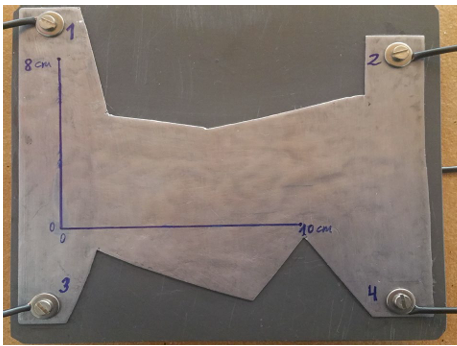
\includegraphics[width=0.9\linewidth]{Agros/placa prueba.png}
	\caption{imagen de la placa dentada que vamos a usar con los diferentes terminales.}
	\label{Fig:01}
\end{subfigure}
\begin{subfigure}{0.45\linewidth} \centering
	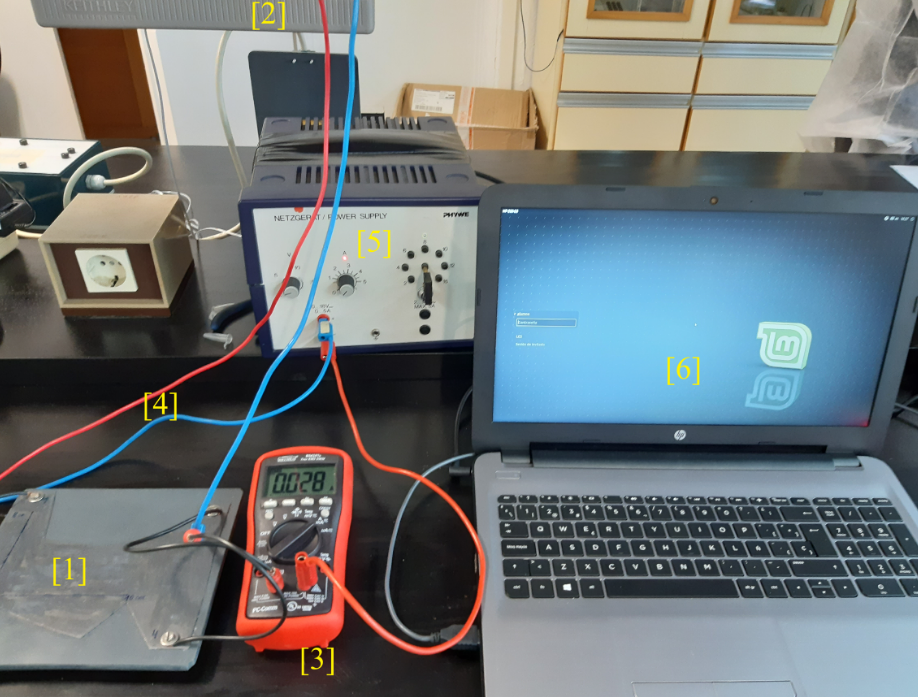
\includegraphics[width=0.9\linewidth]{Agros/Disposicion.png}
	\caption{diposición usada en el experimento (foto de Ivan Cambón \cite{IvanCambon}).}
	\label{Fig:02}
\end{subfigure}
\caption{}
\end{figure}

Como realizamos la digitalización o la simulación es, ciertamente, innecesario, ya que todo lo que realizamos está en el guión de la práctica \cite{Guion}.

%\subsection{Notación de las disposiciones}

%Para denotar las disposiciones de ahora en adelante vamos a usar el siguiente código. Denotamos por disposición a $I(a,b)V(c,d)$ donde $a,b,c,d$ son números del 1 al 4, que corresponderán a las entradas y salidas de voltaje. Por ejemplo, $I(1,4)V(2,3)$ indica que $I^+$ estaba en la terminal 1, $I^-$ en 4, $V^+$ en 2 y $V^-$ en 3 \cite{IvanCambon}.


\section{Incertidumbres}

En esta práctica en particular el tema de las incertidumbres es bastante delicado, ya que la mayor fuente de incertidumbres es la parametrización de los terminales dentro de la propia simulación. Los valores medibles que son la intensidad entre dos terminales y la diferencia voltaje entre los otros dos tienen una incertidumbre dada por el polímetro. Por desgracia durante la práctica se nos estropeo el polímetro, por lo que tuvimos que usararios de diferentes prácticas a medida que nuestros compañeros dejaban libres unos u otros. Consecuentemente no tenemos un valor de incertidumbre único y general, lo que escala la dificultad del análisis de la incertidumbre de los valores experimentales. Para solucionar el problema lo que haremos será coger los valores típicos de un polímetro normal para nuestros valores, que son:

\begin{equation}
	u_B(I) = 1\% \cdot I + 2 \cdot \text{digit} \qquad 	u_B(V) = 0.5\% \cdot V + 2 \cdot \text{digit} 
\end{equation}
Dado que todas las medidas son únicas (no realizamos análisis estadístico de cada voltaje) tenemos que $u(V_{\exp})=u_B(V_{\exp})$ y $u(I_{\exp})=u_B(I_{\exp})$.

Ahora bien, el otro valor que afectará a nuestra incertidumbre $\Delta V_{\simu}$. Para calcular esta lo que haremos será medir coger voltajes cerca de la terminal en la simulación ($V_+,V_-$, indicados sin el subíndice sim por comodidad), alrededor de la termial lo más separados posibles, y realizar una media de todos estos. La incertidumbre  del valor medio será: 

\begin{equation}
	u(\overline{V_\pm}) = u_A(\overline{V_\pm}) = \sqrt{\frac{\sum_j^N (V_{\pm i} - \overline{ V_\pm})^2}{(N-1)N}}
\end{equation}
siendo solo de tipo A ya que cada medida no tiene una incertidumbre de tipo V asignable (al menos nosotros, que no conocemos como funciona la simulación Agross) y luego simplemente propagamos incertidumbres:

\begin{equation}
	\Delta V_{\simu} = {\overline{V_+} - ,\overline{V_-}}  \qquad u(\Delta V_{\simu})  = \sqrt{u(V_+)^2 + u(V_-)^2}
\end{equation}
Sin embargo esto es un poco fútil ya que la mayor fuente de incertidumbre es la parametrización de las terminales (en particular de su tamaño y su distancia con los bordes de la placa metálica). Para obtener la inceritdumbre de $\sigma$ y $\rho$ hemos hecho la clásica fórmula de la \textit{propagación de incertidumbre} que podemos ver en cualquier manual de estadística y de análisis de incertidumbres. Nosotros usamos como referencia \cite{Estadistica}.


Como la distancia entre el borde de la placa metálica y la terminal es conocida no tenemos que hacer un estudio moviendo este a lo largo de la práctica. Tampoco hace falta hacer varios radios, ya que los valores máximo y mínimo del radio estás limitados. El valor máximo del radio vendŕa dada por  el tamaño de la cabeza del tornillo ($r=0.390$ cm), ya que <<siendo la arandela el tamaño máximo que tiene el agujero, es lógico pensar que dará la variación máxima debida al tamaño del contacto con respecto al de la cabeza del tornillo>> (Carballeira Romero Carlos), y por otro lado nos quedamos con un valor medio entre el la cabeza del tornillo y la arandela ($r=0.31$ cm). Por desgracia no medimos en el laboratorio el tamaño más pequeño posible, que sería justo del tamaño del vástago del tornillo y más pequeño que la cabeza, por lo que nos tenemos que conformar solo con dos modelizaciones. 

\section{Material óhmico} \label{Sec:04}

Como podemos ver en las gráficas los resultados obtenidos indican un comportamiento claramente lineal entre intensidad y voltaje. En las gráficas representamos los puntos experimentales y el ajuste lineal, con los parámetros incluidos en la propia gráfica tal que: 

\begin{equation}
	y(x) = p_0 + p_1 \cdot x
\end{equation}
concluyendo que efectivamente se comporta como un \textbf{material óhmico} y que por tanto podemos obtener $\sigma_{\exp}$ a través del desarrollo teórico. 

\begin{figure}[h!]
	\caption{Representación de $V$ frenta $I$ y regresión lineal de cada una de las disposiciones.}
	\label{Fig:03}
	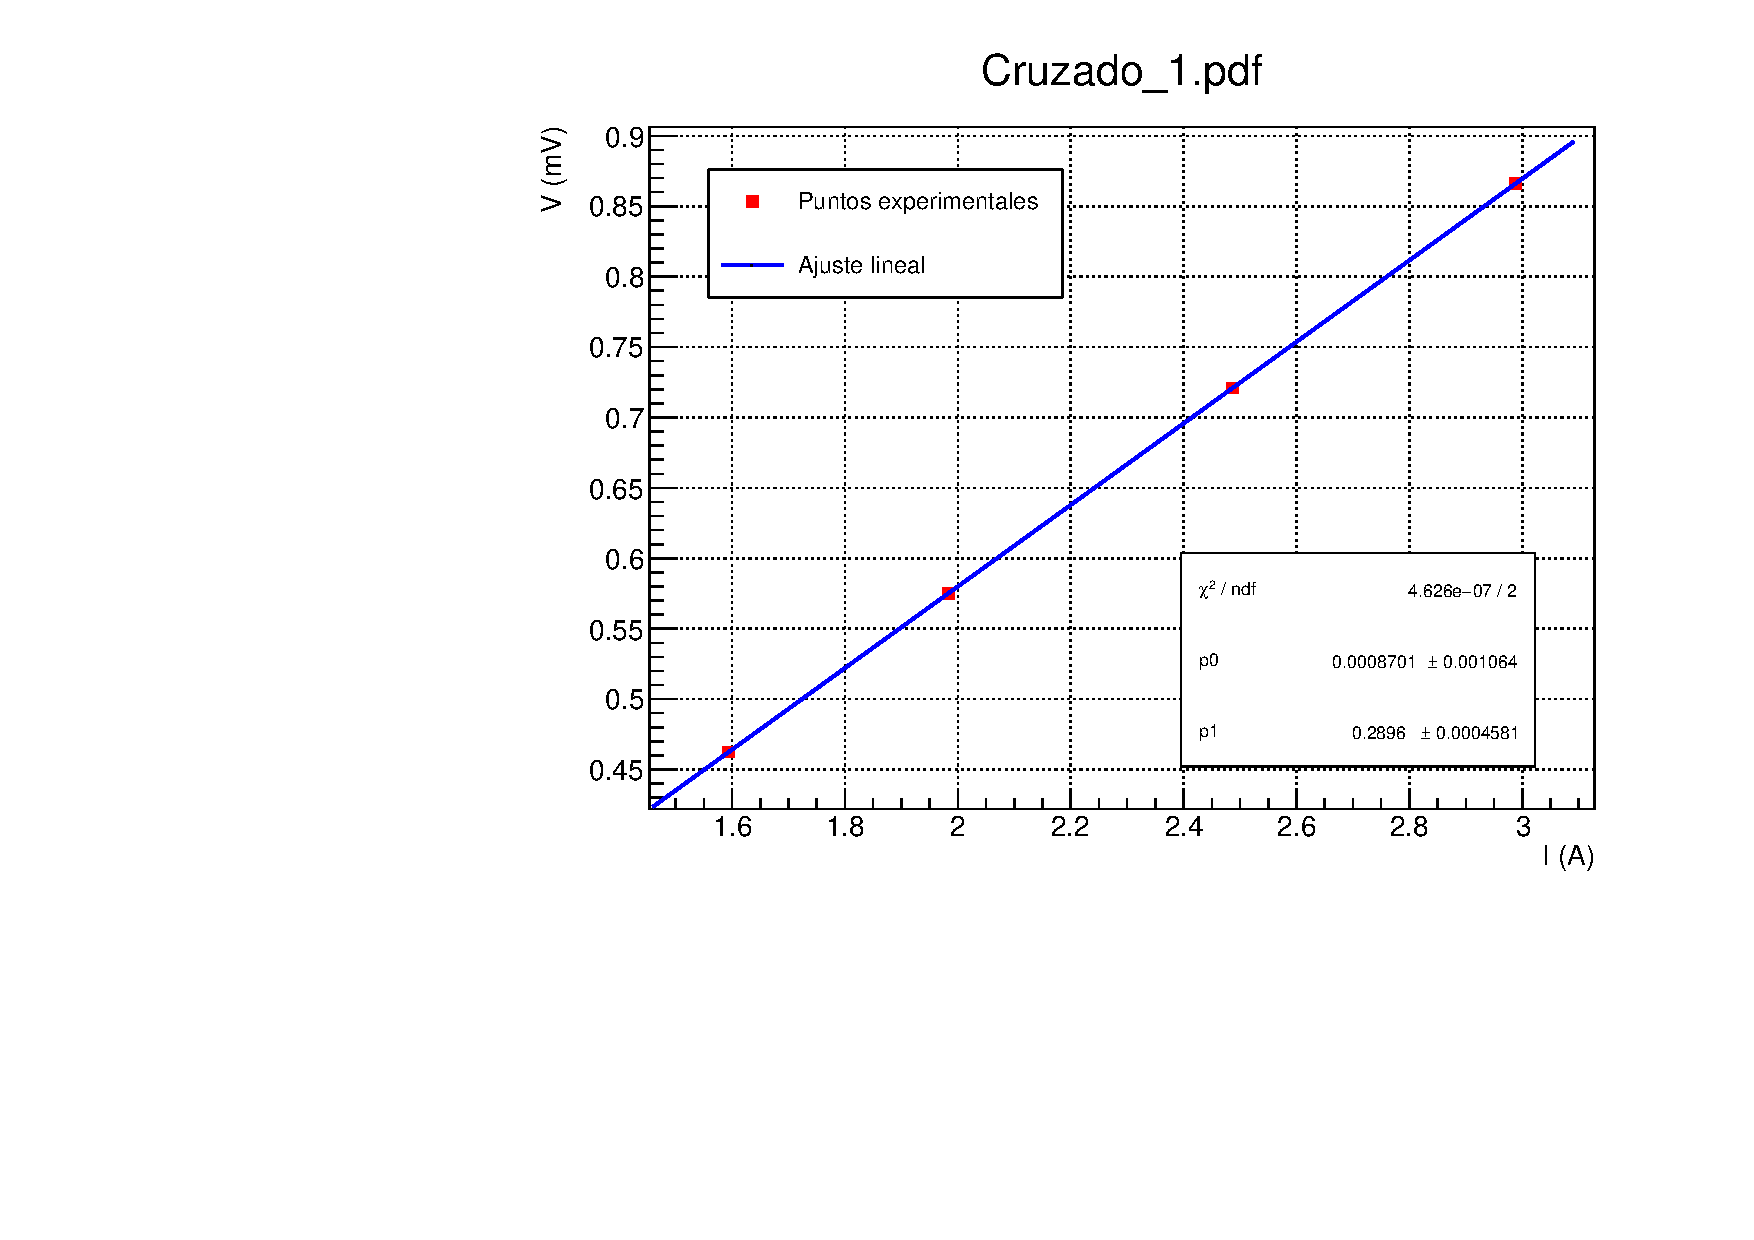
\includegraphics[width=0.5\linewidth]{Programas/Cruzado_1.pdf} \hfill
	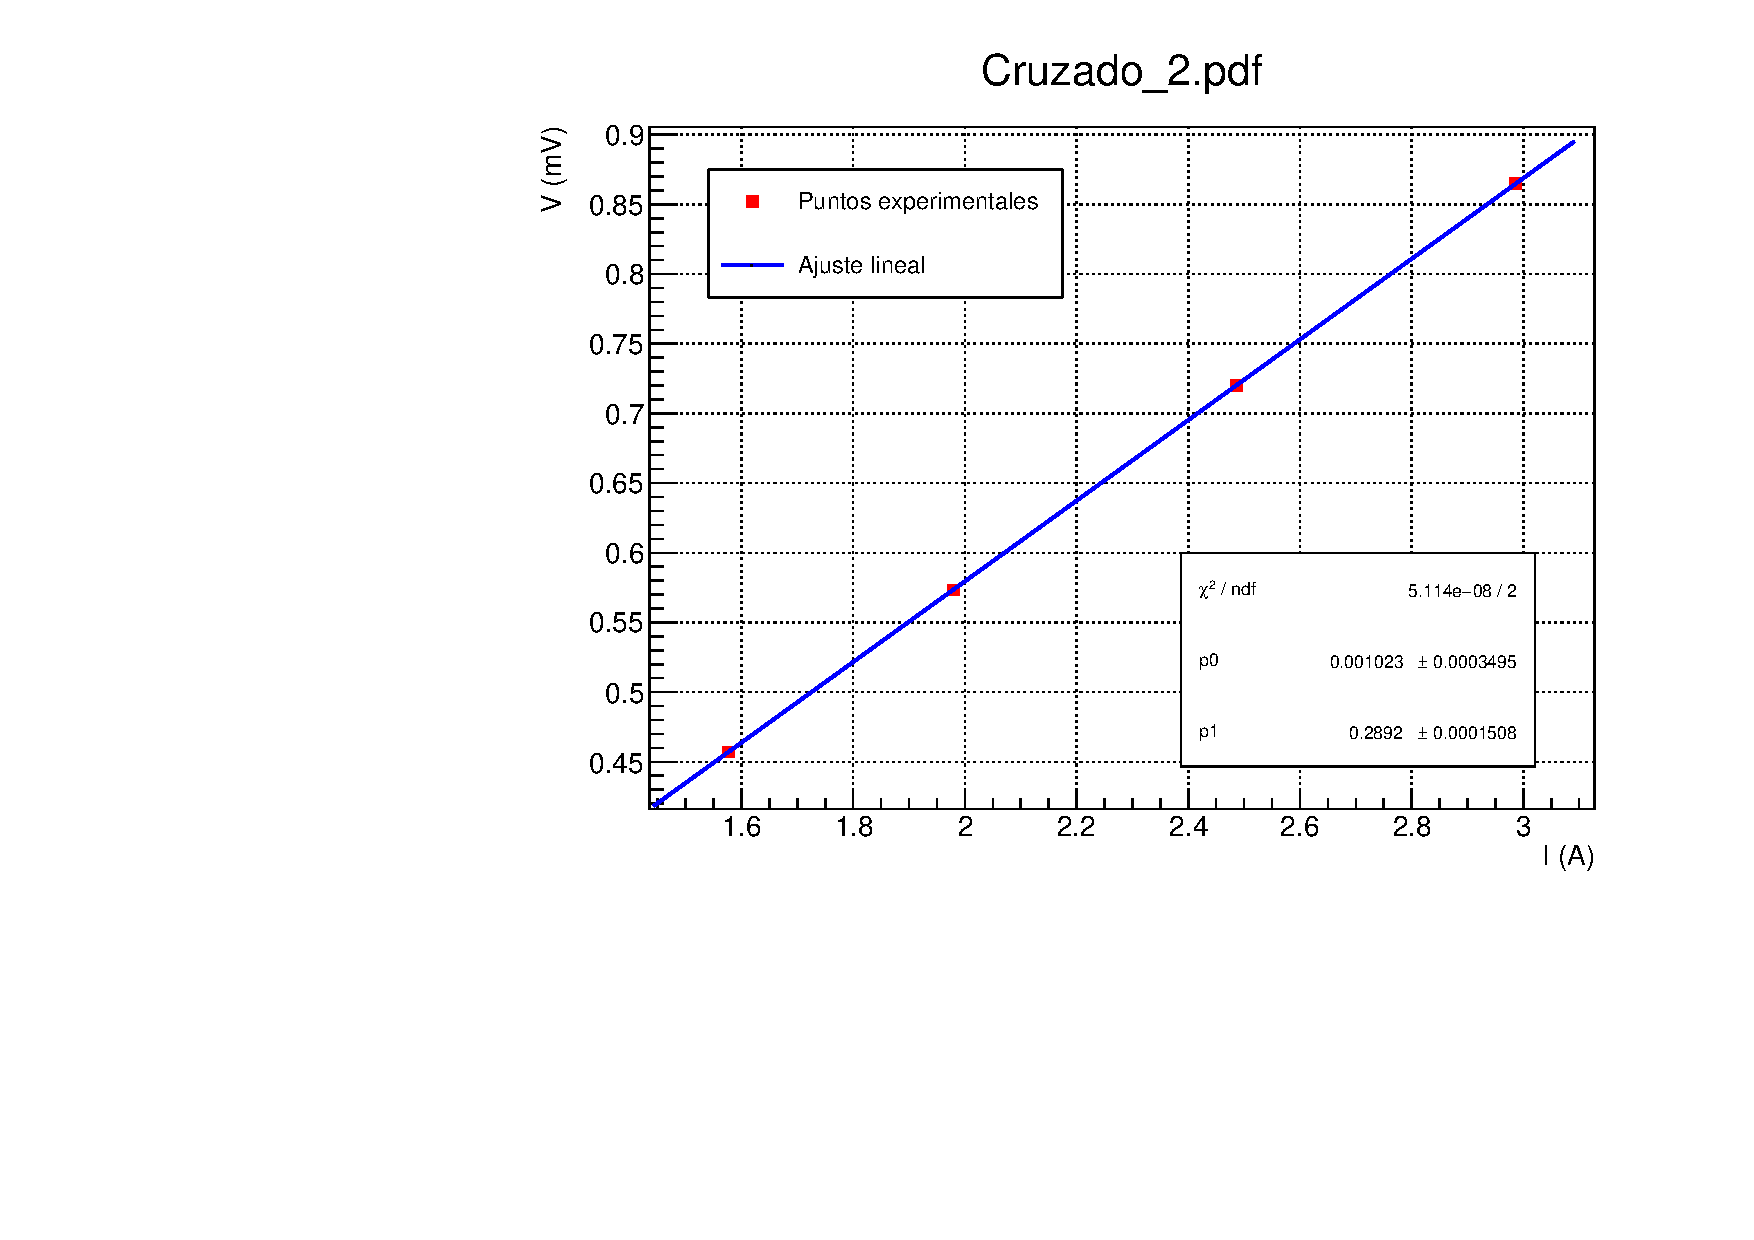
\includegraphics[width=0.5\linewidth]{Programas/Cruzado_2.pdf}
\end{figure}
\begin{figure}[h!]
	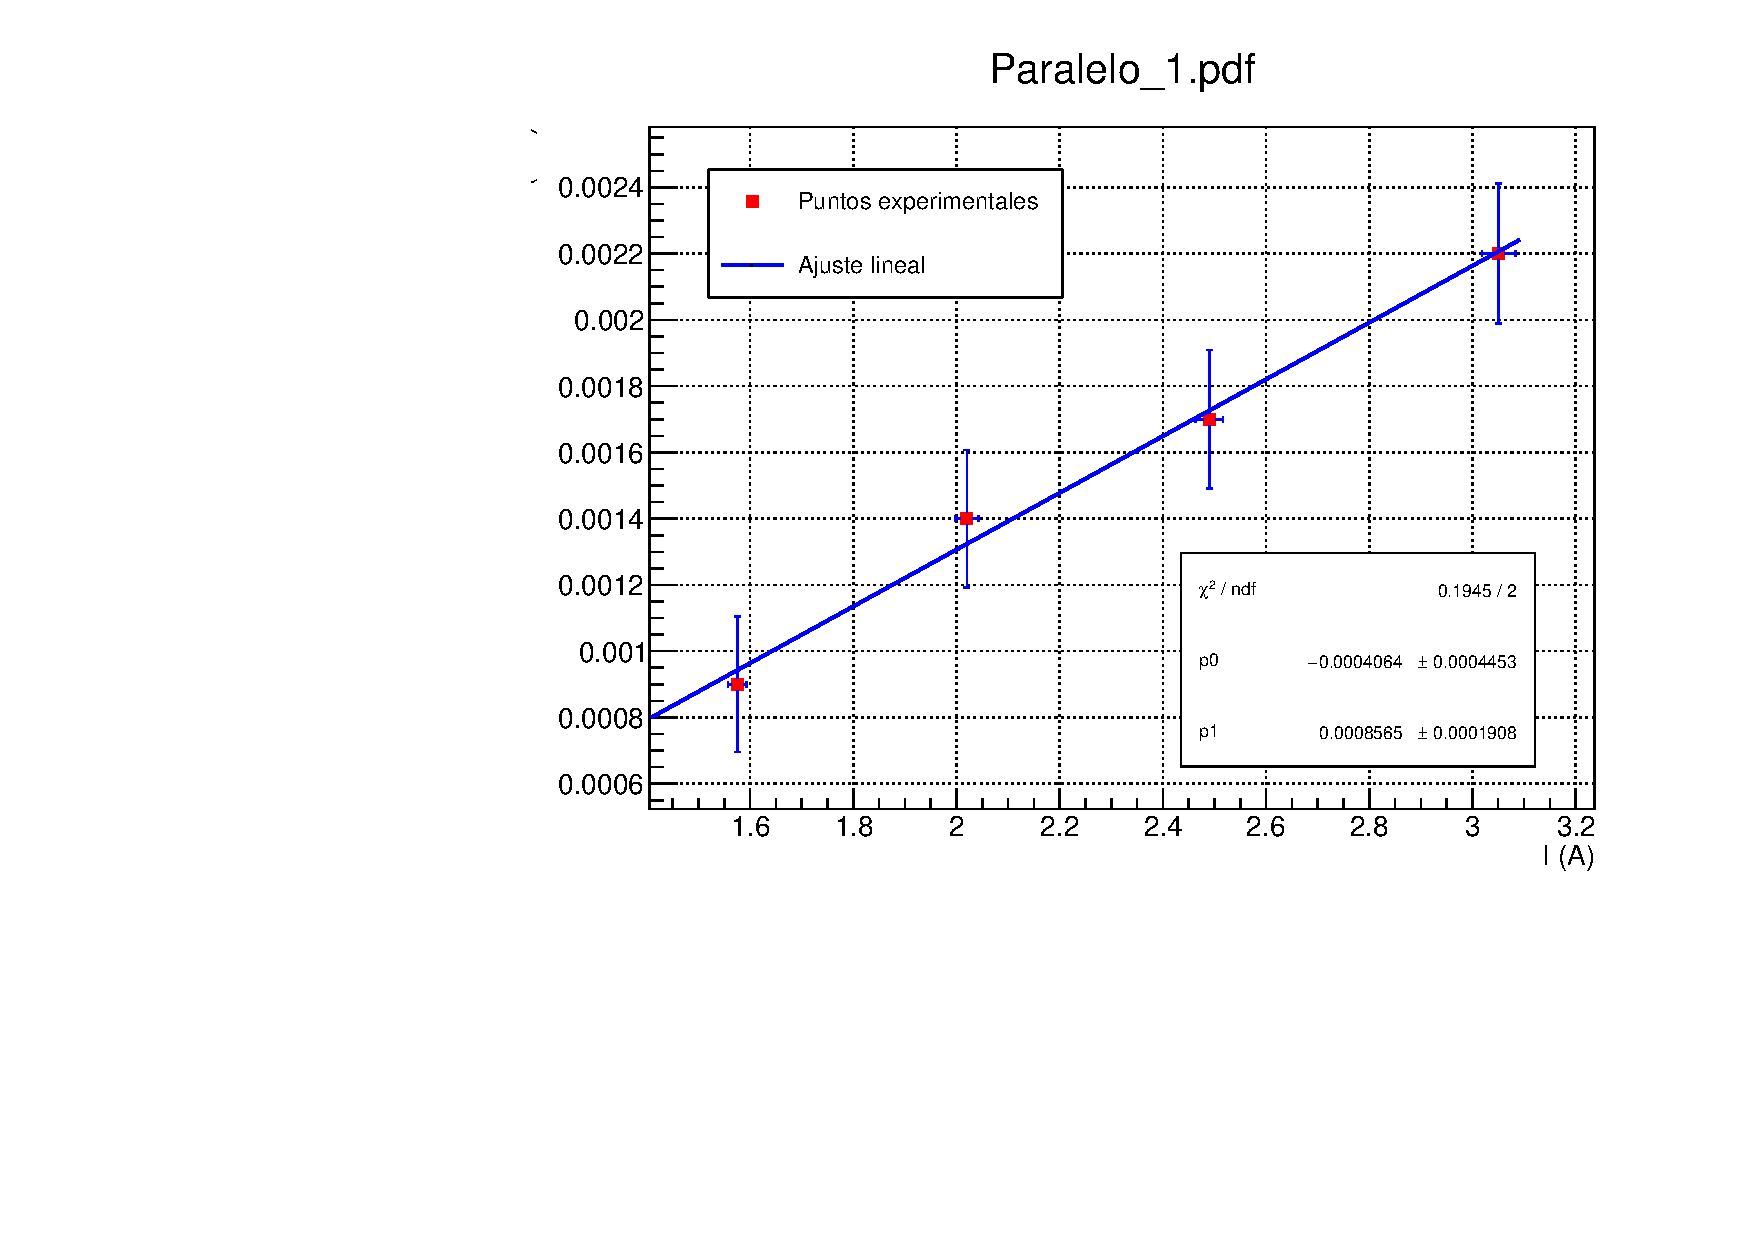
\includegraphics[width=0.5\linewidth]{Programas/Paralelo_1.pdf} \hfill
	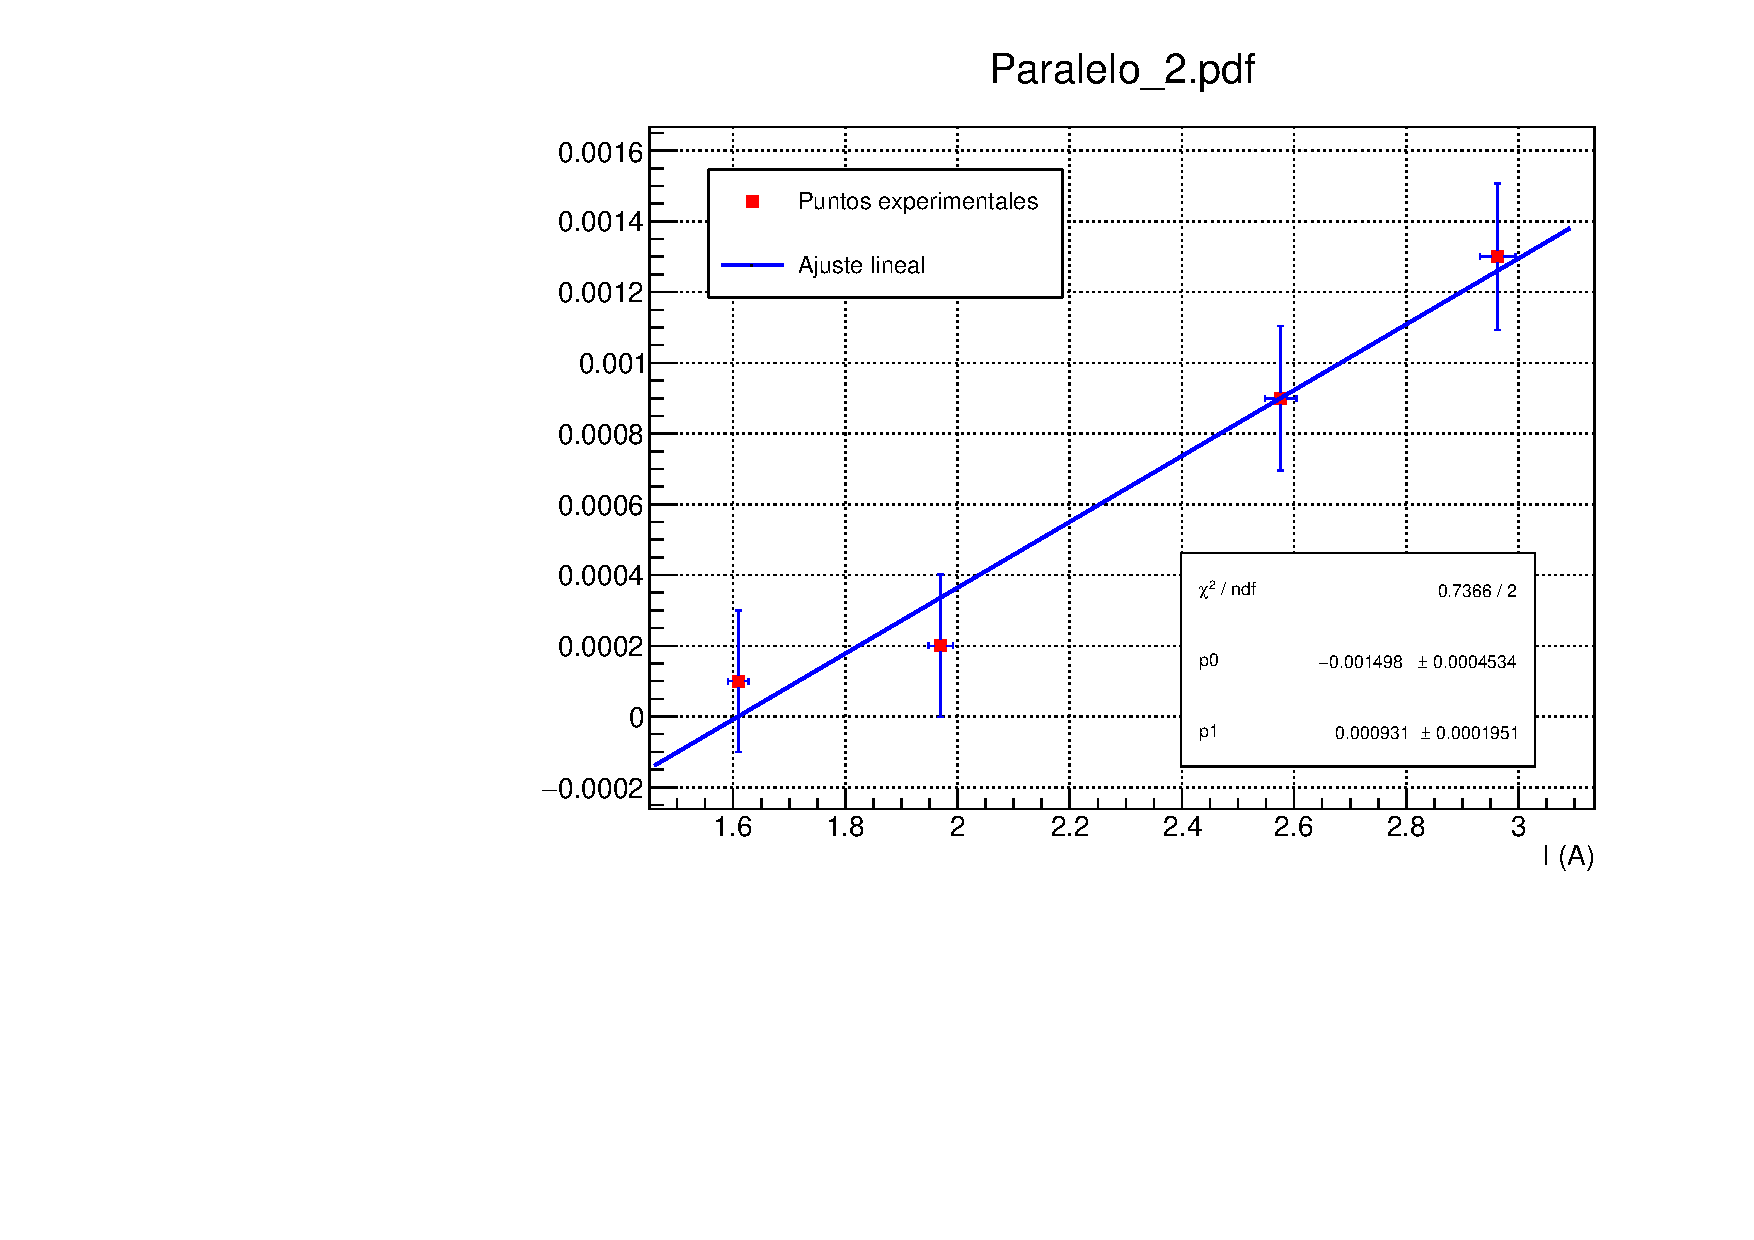
\includegraphics[width=0.5\linewidth]{Programas/Paralelo_2.pdf}
\end{figure}
\begin{figure}[h!]
	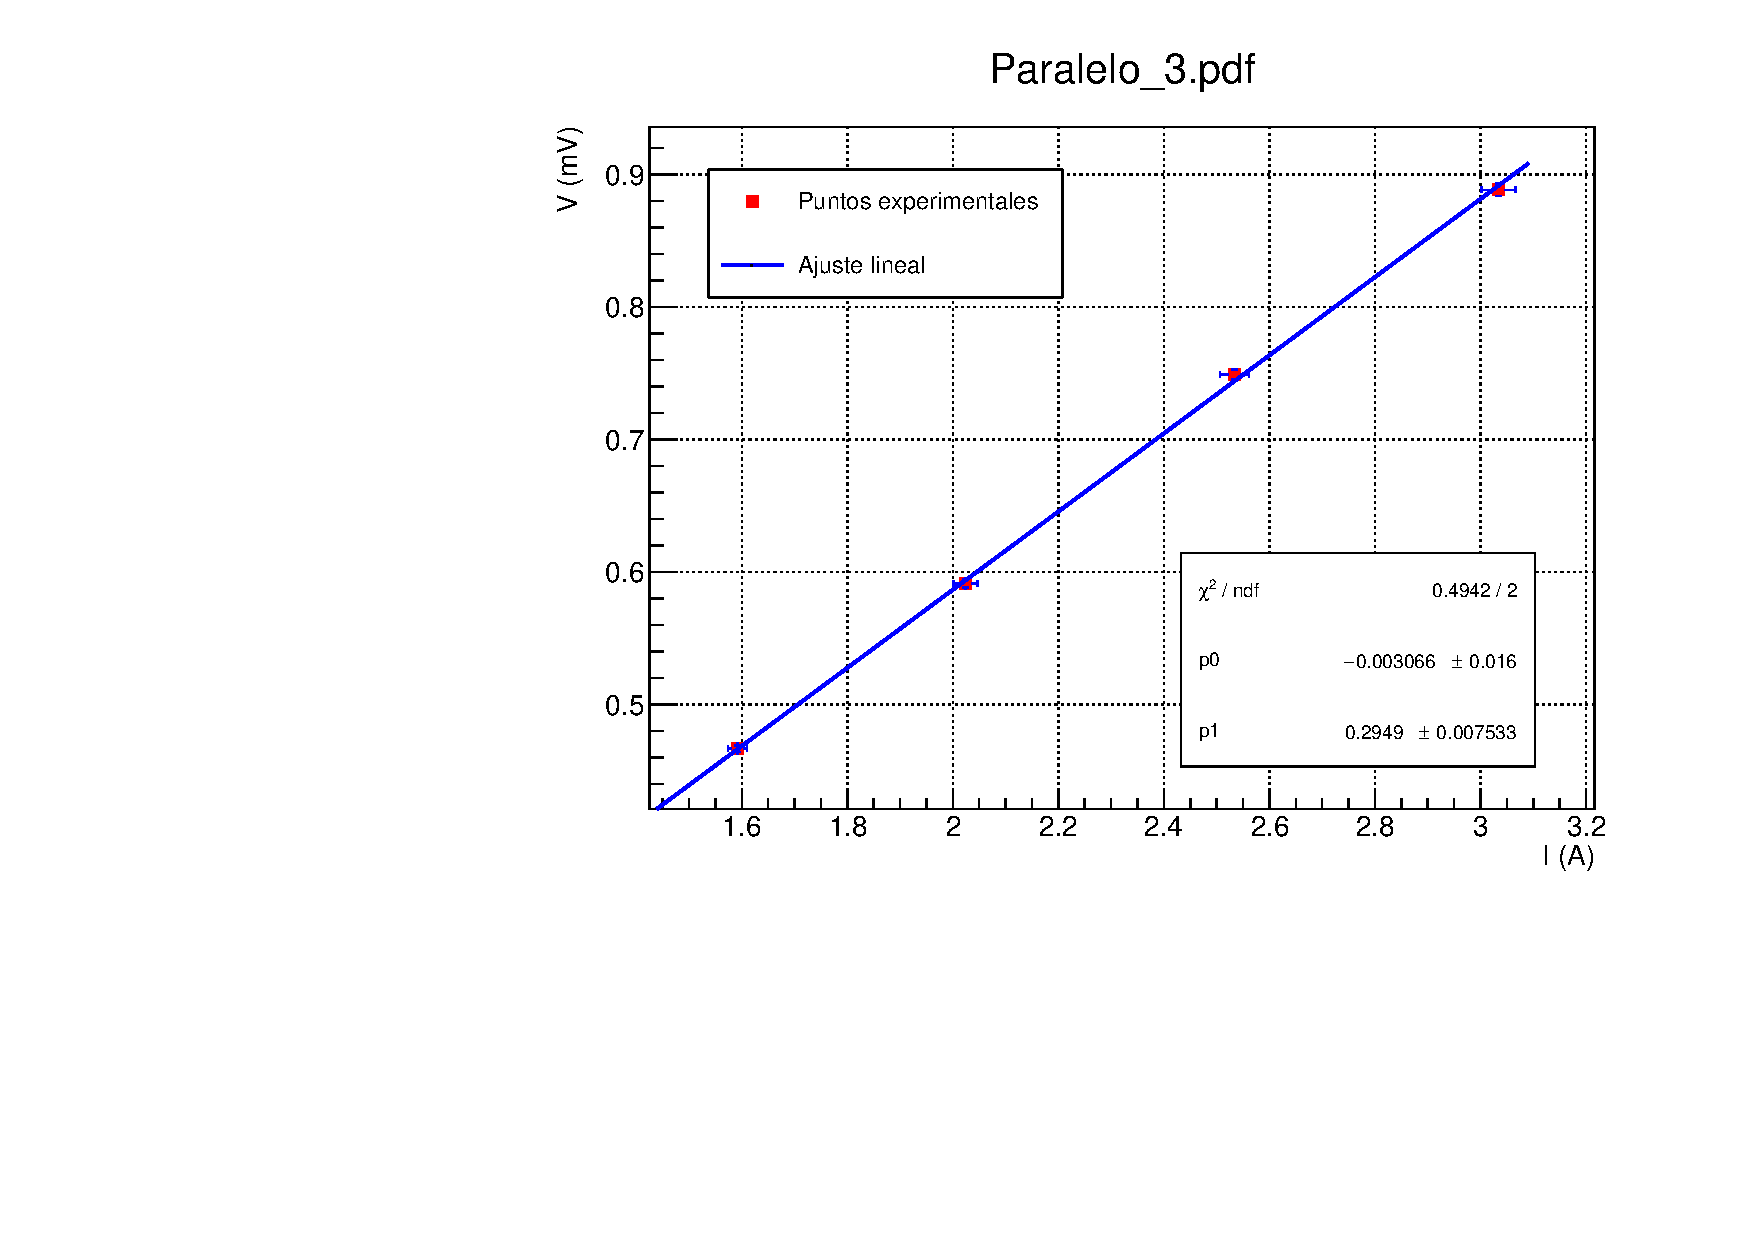
\includegraphics[width=0.5\linewidth]{Programas/Paralelo_3.pdf} \hfill
	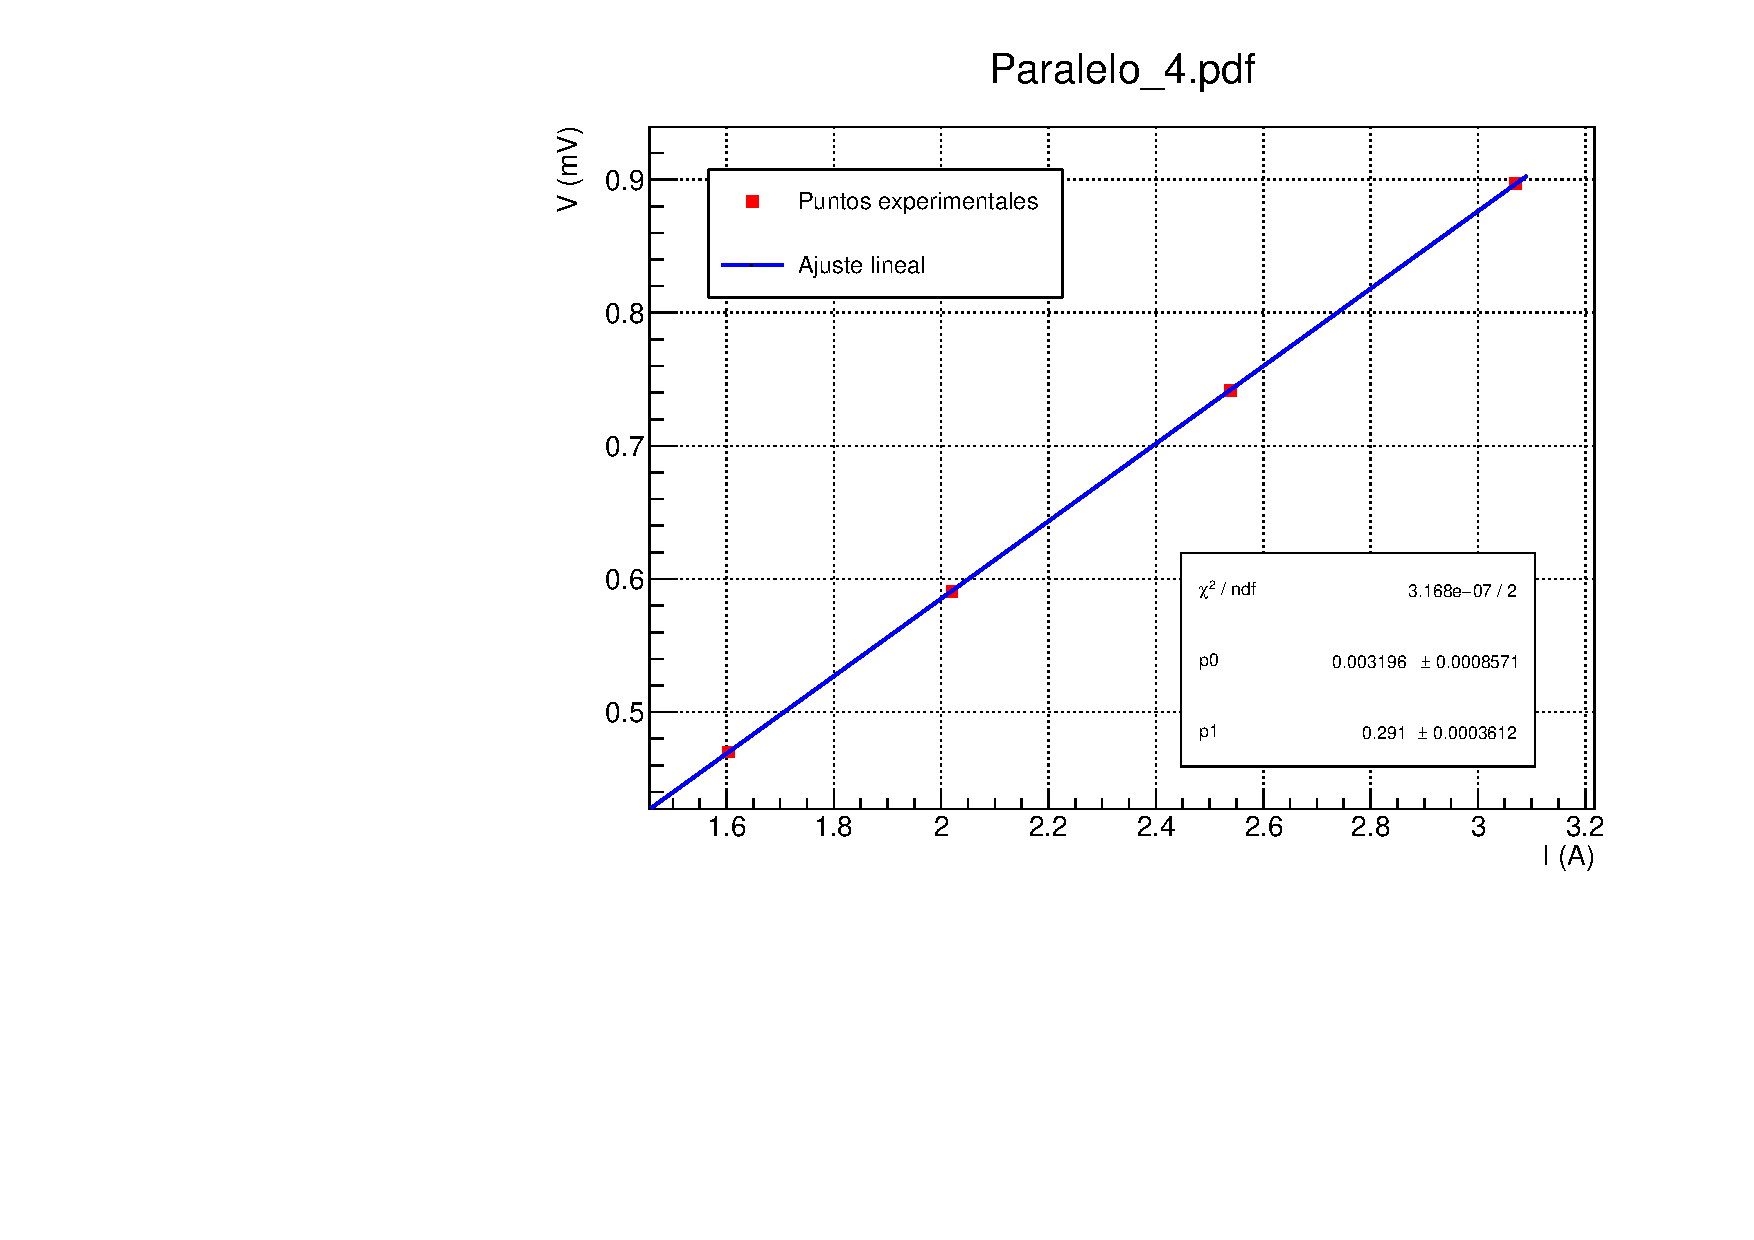
\includegraphics[width=0.5\linewidth]{Programas/Paralelo_4.pdf}
\end{figure}

Como podemos ver $\chi^2/$ndf (en las imagenes \ref{Fig:03}) es simpre menor que uno, siendo extremadamente pequeña para los datos de las disposiciones 1,2,5 y 6, lo cual era lo esperable ya que tienen el mejor comportamiento, mientaras que para 3 y 4 el comportamiento se desvía un poco más aunque no lo suficiente para afirmar que no tiene un comportamiento óhmico. Los datos usados (y las correspondientes incertidumbres) las podemos encontrar en el apéndice \ref{Appendix:A}. Las $\chi^2/$ndf las hemos obtenido a través de los programas de C++ CERN ROOT \cite{Root}, que podéis visitar en \url{https://root.cern/}. Los resultados mostrados nos permiten afirmar que \textit{los datos obtenidos concuerdan con una distribución lineal, i.e., que los datos avalan un comportamiento óhmico del material usado en la práctica}.



\section{Calculo de la resistivdad del material}

Como ya hemos indicado, nosotros vamos a medir voltajes para una entrada particular de intensidad, queriendo calcular la resisitivdad del material, por lo que la información importante será $(V_{\exp},\sigma_{\exp})$, siendo $\sigma_{\exp}$ la que queremos calcular. Los valores que nos va a dar la simulación son pares de $(V_{\simu},\sigma_{\simu}$) siendo la intensidad $I_{\exp}$ y $I_{\simu}$ iguales, en una experimental y en otra un parámetro que introducimos a mano. Dado que la ley de Ohm $V\varpropto \rho = 1 / \sigma$ que hemos comprobado que el material sigue (sección \ref{Sec:04}), podemos suponer que $V\times \sigma = \cte$, y por tanto se debe verificar que: 

\begin{equation}
	V_{\exp} \times \sigma_{\exp} = V_{\simu} \times \sigma_{\simu}
\end{equation}
tal que: 

\begin{equation}
	\sigma_{\exp} =  \frac{V_{\simu}}{V_{exp}} \times \sigma_{\simu}
\end{equation}
Recordamos que la \textbf{conductividad} $\sigma$ se mide en $[S / m]$ y que su inversa es la \textbf{resistividad} denotada por $\rho$:

\begin{equation}
	\rho = \frac{1}{\sigma}
\end{equation}
que se mide en $[\Omega \cdot $ m]. Tomaremos $\sigma_{\simu}=3\cdot 10^5$ S/m.

La intensidad que nosotros medimos en el lab no es igual al parámetro que nos pide Agross (progrma que realiza la simulación). El funcionamiento de la misma es un poco complicada, ya que modeliza una terminal como un círculo formado por 4 segmentos, de tal modo que nosotros tenemos que introducir la corriente por segmento, así pues el $I$ que vamos a introducir está divido por 4. Sin embargo todavía falta algo, ya que Agross no pide el valor de la intensidad $I$ en amperios tal y como medimos nosotros en el laboratorio, tenemos que darle el valor de la densidad de corriente $J [\unit{A/m^2}]$ introducida por los terminales, por lo que vamos a introducir el valor de $I$ dividido entre 4 y por el espesor y el tamaño de uno de los segmentos. Si $r$ es el radio, veamos que:

\begin{equation}
	J = \frac{I}{2 \pi r d}
\end{equation}
Por suerte el espesor $d$ nos lo dan en el guión y lo tomaremos por un valor constante sin incertidumbre:
\begin{equation}
	d = 1 \ \unit{mm}
\end{equation}
Dado que la longitud de cada segmento (o radio) dependerá de la modelización, y eso variará en función de la parte de la práctica en la que estemos, ya que como veremos, es una de las grandes fuentes de incertidumbre, tendremos que indicarlo en cada momento.


\section{Resultados}

Los resultados los evaluaremos disposición a disposición para ambas parametrizaciones $r_1=0.313$ cm y $r_2=0.390$ cm. Las densidades de corrientes las denotamos por $J_1\equiv J(r_1)$ y $J_2\equiv J(r_2)$. En la disposición 1 iremos comentando un poco los resultados, mientras que para las disposiciones posteriores evitaremos realizar estos comentarios (ya que sería repetirlos 6 veces). Así pues: 


\subsection{Disposición 1}


Los valores experimentales tal que $\Delta V_{\exp}$, $I_{\exp}$ y $J_{1\exp}$  y $J_{2\exp}$ son:

\begin{table}[H]
    \centering
\begin{tabular}{cccc}
\toprule
$I$ [A] & $V$ [V] & $J_1$ [A/cm$^2$] & $J_2$ [A/cm$^2$] \\
\midrule
2.988 $\pm$ 0.032 & 0.8660 $\pm$ 0.0045 & 15.18 $\pm$ 0.15 & 12.19 $\pm$ 0.12 \\
\bottomrule
\end{tabular}
    \caption{Tabla de la valores para la disposición 1 $r_1=0.313$ y $r_2=0.390$ cm }
    \label{Tab:VIJ_mini_1}
\end{table}

Dado que no podemos calcular directamente $\Delta V_{\simu}$ ya que alrededor de las terminales varía un poco el voltaje (véase imagen) tal que mediremos varios $V_+$ y $V_-$ simulados, obteniendo una media (y su incertidumbre, tal y como hemos indicado arriba) tal que $\Delta V_{\simu} = \overline{V}_+ - \overline{V}_{-} $. Así pues: 

\begin{table}[H]
    \centering
\begin{tabular}{c|cccc|ccc}
\toprule
\midrule
$V_+$ [mV] & \SI{3.075e-01}{} & \SI{3.069e-01}{} & \SI{3.077e-01}{} & \SI{3.072e-01}{} & $\overline{V}_+$ [$\mu$V] & $\overline{V}_-$ [$\mu$V] & $\Delta V_{\simu}$ [$\mu$V] \\
$V_-$ [mV] & \SI{0.1733}{} & \SI{0.1733}{} & \SI{0.1733}{} & \SI{0.1733}{} & \SI{173.30}{} & \SI{307.33}{} $\pm$ 0.18 & \SI{134.03}{} $\pm$ 0.18 \\
\bottomrule
\end{tabular}
    \caption{Tabla de la valores para la disposición 1 de $V_+$ y $V_-$ con r=0.31 cm}
    \label{Tab:Vpn1_1}
\end{table}

\begin{table}[H]
    \centering
\begin{tabular}{c|cccc|ccc}
\toprule
\midrule
$V_+$ [mV] & \SI{3.027e-01}{} & \SI{3.029e-01}{} & \SI{3.024e-01}{} & \SI{3.020e-01}{} & $\overline{V}_+$ [$\mu$V] & $\overline{V}_-$ [$\mu$V] & $\Delta V_{\simu}$ [$\mu$V] \\
$V_-$ [mV] & \SI{0.1685}{} & \SI{0.1685}{} & \SI{0.1685}{} & \SI{0.1685}{} & \SI{168.50}{} & \SI{302.50}{} $\pm$ 0.20 & \SI{134.00}{} $\pm$ 0.20 \\
\bottomrule
\end{tabular}
    \caption{Tabla de la valores para la disposición 1 de $V_+$ y $V_-$ con r=0.39 cm}
    \label{Tab:Vpn2_1}
\end{table}

y el valor de la resistividad es, para cada parametrización del radio: \\[1em]
\begin{minipage}[t]{0.45\linewidth} 
	\begin{center}
	\captionof{table}{Valores de $\sigma$ y $\rho$ para $r=0.313$ cm.}
	\vspace{0.5em}
	\begin{tabular}{ccc}
\toprule
$\sigma_{\exp}$ [S/cm] & $\rho_{\exp}$ [$\Omega  \cdot$cm] \\
\midrule
\num{46428.984(250.320)} & \num{0.00002154(0.00000012)} \\
\bottomrule
\end{tabular}

	\vspace{1.2em}
	\captionof{table}{Valores de $\sigma$ y $\rho$ para $r=0.390$ cm.}
	\vspace{0.5em}
	\begin{tabular}{ccc}
\toprule
$\sigma_{\exp}$ [S/cm] & $\rho_{\exp}$ [$\Omega$cm] \\
\midrule
\num{46420.323(252.117)} & \num{0.00002154(0.00000012)} \\
\bottomrule
\end{tabular}

	\end{center}  
\end{minipage}
\hfill
\begin{minipage}[t]{0.45\linewidth}
	\begin{center}
	\captionof{figure}{Campo escalar para la disposición 1 con $r_1$.}
	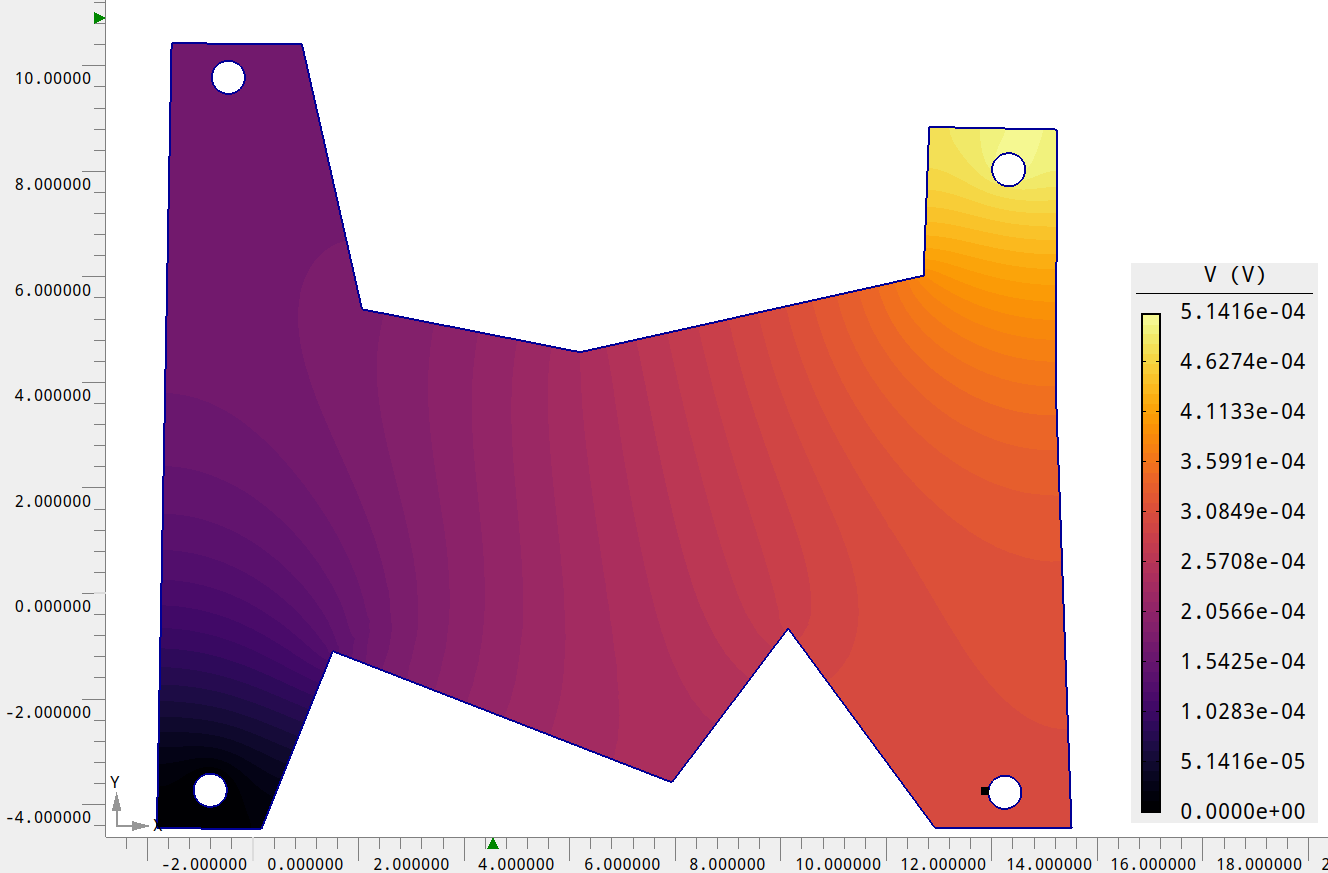
\includegraphics[width=1\linewidth]{Imagen Agros 1/Agros1.png}
	\end{center}  	
\end{minipage} \\[2em]
La imagen de la derecha representa el campo escalar para la disposición 1 para el radio $r_1$. 

\subsection{Disposición 2}

Los valores de los diferentes parámetros en la disposición 2 son: 
\begin{table}[H]
    \centering
\begin{tabular}{cccc}
\toprule
$I$ [A] & $V$ [V] & $J_1$ [A/cm$^2$] & $J_2$ [A/cm$^2$] \\
\midrule
2.986 $\pm$ 0.032 & 0.8648 $\pm$ 0.0045 & 15.17 $\pm$ 0.15 & 12.18 $\pm$ 0.12 \\
\bottomrule
\end{tabular}
    \caption{Tabla de la valores para la disposición 2 $r_1=0.313$ y $r_2=0.390$ cm }
    \label{Tab:VIJ_mini_2}
\end{table}

\begin{table}[H]
    \centering
\begin{tabular}{c|cccc|ccc}
\toprule
\midrule
$V_+$ [mV] & \SI{3.499e-01}{} & \SI{3.500e-01}{} & \SI{3.501e-01}{} & \SI{3.501e-01}{} & $\overline{V}_+$ [$\mu$V] & $\overline{V}_-$ [$\mu$V] & $\Delta V_{\simu}$ [$\mu$V] \\
$V_-$ [mV] & \SI{0.2161}{} & \SI{0.2162}{} & \SI{0.2160}{} & \SI{0.2160}{} & \SI{216.08}{} $\pm$ 0.05 & \SI{350.03}{} $\pm$ 0.05 & \SI{133.95}{} $\pm$ 0.07 \\
\bottomrule
\end{tabular}
    \caption{Tabla de la valores para la disposición 2 de $V_+$ y $V_-$ con r=0.31 cm}
    \label{Tab:Vpn1_2}
\end{table}

\begin{table}[H]
    \centering
\begin{tabular}{c|cccc|ccc}
\toprule
\midrule
$V_+$ [mV] & \SI{3.450e-01}{} & \SI{3.449e-01}{} & \SI{3.451e-01}{} & \SI{3.452e-01}{} & $\overline{V}_+$ [$\mu$V] & $\overline{V}_-$ [$\mu$V] & $\Delta V_{\simu}$ [$\mu$V] \\
$V_-$ [mV] & \SI{0.2111}{} & \SI{0.2110}{} & \SI{0.2112}{} & \SI{0.2114}{} & \SI{211.18}{} $\pm$ 0.09 & \SI{345.05}{} $\pm$ 0.06 & \SI{133.87}{} $\pm$ 0.11 \\
\bottomrule
\end{tabular}
    \caption{Tabla de la valores para la disposición 2 de $V_+$ y $V_-$ con r=0.39 cm}
    \label{Tab:Vpn2_2}
\end{table}


\begin{minipage}[t]{0.45\linewidth} 
	\begin{center}
	\captionof{table}{Valores de $\sigma$ y $\rho$ para $r=0.313$ cm.}
	\vspace{0.5em}
	\begin{tabular}{ccc}
\toprule
$\sigma_{\exp}$ [S/cm] & $\rho_{\exp}$ [$\Omega  \cdot$cm] \\
\midrule
\num{46467.391(244.215)} & \num{0.00002152(0.00000011)} \\
\bottomrule
\end{tabular}

	\vspace{1.2em}
	\captionof{table}{Valores de $\sigma$ y $\rho$ para $r=0.390$ cm.}
	\vspace{0.5em}
	\begin{tabular}{ccc}
\toprule
$\sigma_{\exp}$ [S/cm] & $\rho_{\exp}$ [$\Omega  \cdot$cm] \\
\midrule
\num{46441.374(245.769)} & \num{0.00002153(0.00000011)} \\
\bottomrule
\end{tabular}

	\end{center}  
\end{minipage}
\hfill
\begin{minipage}[t]{0.45\linewidth}
	\begin{center}
	\captionof{figure}{Campo escalar para la disposición 2 con $r_1$.}
	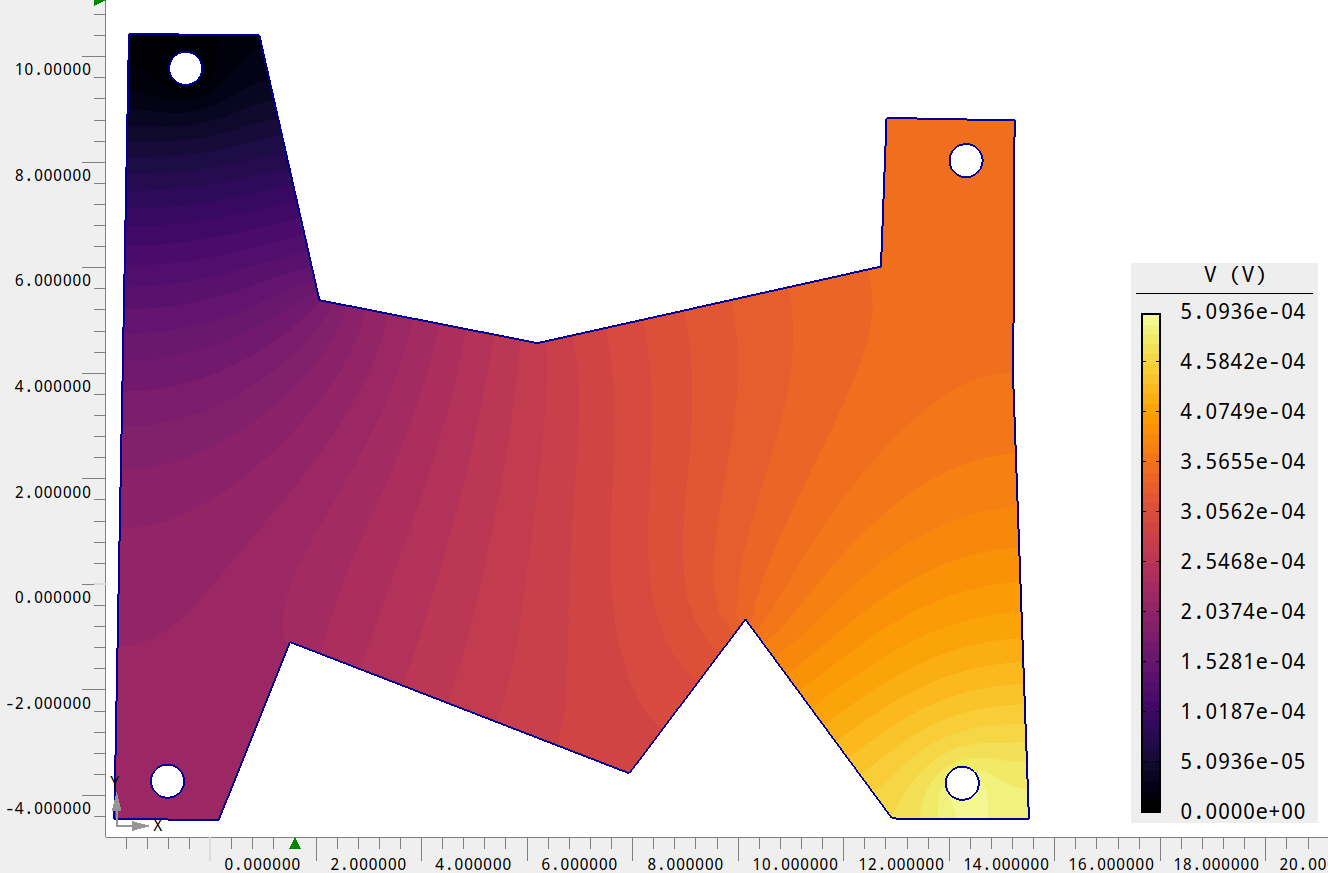
\includegraphics[width=1\linewidth]{Imagen Agros 1/Agros2.png}
	\end{center}  	
\end{minipage}

\subsection{Disposición 3}

\begin{table}[H]
    \centering
\begin{tabular}{cccc}
\toprule
$I$ [A] & $V$ [V] & $J_1$ [A/cm$^2$] & $J_2$ [A/cm$^2$] \\
\midrule
3.051 $\pm$ 0.033 & 0.0022 $\pm$ 0.0002 & 15.50 $\pm$ 0.16 & 12.44 $\pm$ 0.13 \\
\bottomrule
\end{tabular}
    \caption{Tabla de la valores para la disposición 3 $r_1=0.313$ y $r_2=0.390$ cm }
    \label{Tab:VIJ_mini_3}
\end{table}


\begin{table}[H]
    \centering
\begin{tabular}{c|cccc|ccc}
\toprule
\midrule
$V_+$ [mV] & \SI{2.203e-01}{} & \SI{2.203e-01}{} & \SI{2.203e-01}{} & \SI{2.203e-01}{} & $\overline{V}_+$ [$\mu$V] & $\overline{V}_-$ [$\mu$V] & $\Delta V_{\simu}$ [$\mu$V] \\
$V_-$ [mV] & \SI{0.2207}{} & \SI{0.2207}{} & \SI{0.2207}{} & \SI{0.2207}{} & \SI{220.70}{} & \SI{220.30}{} & \SI{0.40}{} \\
\bottomrule
\end{tabular}
    \caption{Tabla de la valores para la disposición 3 de $V_+$ y $V_-$ con r=0.31 cm}
    \label{Tab:Vpn1_3}
\end{table}

\begin{table}[H]
    \centering
\begin{tabular}{c|cccc|ccc}
\toprule
\midrule
$V_+$ [mV] & \SI{1.720e-01}{} & \SI{1.720e-01}{} & \SI{1.720e-01}{} & \SI{1.720e-01}{} & $\overline{V}_+$ [$\mu$V] & $\overline{V}_-$ [$\mu$V] & $\Delta V_{\simu}$ [$\mu$V] \\
$V_-$ [mV] & \SI{0.1716}{} & \SI{0.1716}{} & \SI{0.1716}{} & \SI{0.1716}{} & \SI{171.60}{} & \SI{172.00}{} & \SI{0.40}{} \\
\bottomrule
\end{tabular}
    \caption{Tabla de la valores para la disposición 3 de $V_+$ y $V_-$ con r=0.39 cm}
    \label{Tab:Vpn2_3}
\end{table}


\begin{minipage}[t]{0.45\linewidth} 
	\begin{center}
	\captionof{table}{Valores de $\sigma$ y $\rho$ para $r=0.313$ cm.}
	\vspace{0.5em}
	\begin{tabular}{ccc}
\toprule
$\sigma_{\exp}$ [S/cm] & $\rho_{\exp}$ [$\Omega  \cdot$cm] \\
\midrule
\num{54545.455(5231.405)} & \num{0.00001833(0.00000176)} \\
\bottomrule
\end{tabular}

	\vspace{1.2em}
	\captionof{table}{Valores de $\sigma$ y $\rho$ para $r=0.390$ cm.}
	\vspace{0.5em}
	\begin{tabular}{ccc}
\toprule
$\sigma_{\exp}$ [S/cm] & $\rho_{\exp}$ [$\Omega  \cdot$cm] \\
\midrule
\num{54545.455(5231.405)} & \num{0.00001833(0.00000176)} \\
\bottomrule
\end{tabular}

	\end{center}  
\end{minipage}
\hfill
\begin{minipage}[t]{0.45\linewidth}
	\begin{center}
	\captionof{figure}{Campo escalar para la disposición 3 con $r_1$.}
	\label{Fig:05}
	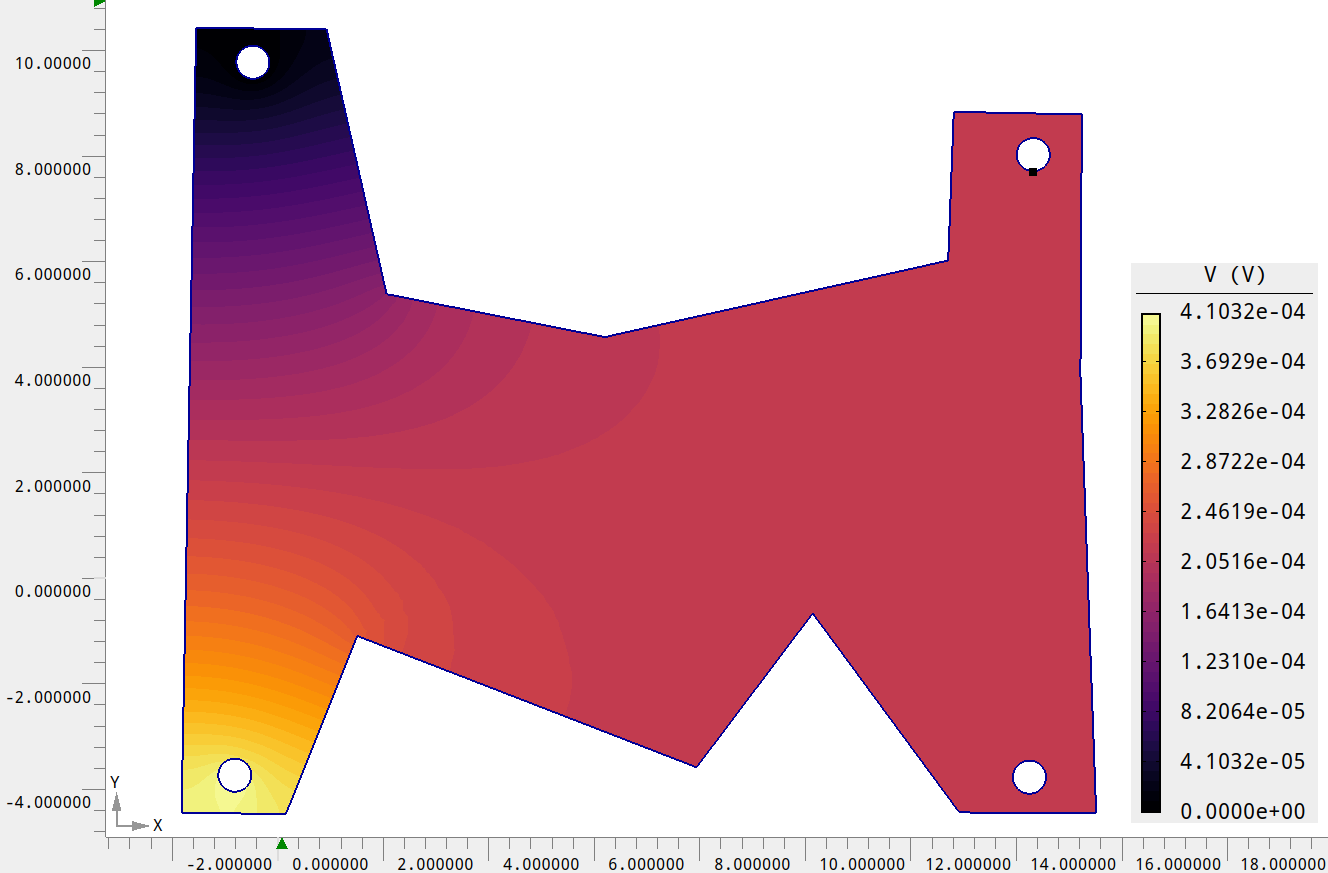
\includegraphics[width=1\linewidth]{Imagen Agros 1/Agros3.png}
	\end{center}  	
\end{minipage}

% Disposición 4
\subsection{Disposición 4}


\begin{table}[H]
    \centering
\begin{tabular}{cccc}
\toprule
$I$ [A] & $V$ [V] & $J_1$ [A/cm$^2$] & $J_2$ [A/cm$^2$] \\
\midrule
2.963 $\pm$ 0.032 & 0.0013 $\pm$ 0.0002 & 15.06 $\pm$ 0.15 & 12.08 $\pm$ 0.12 \\
\bottomrule
\end{tabular}
    \caption{Tabla de la valores para la disposición 4 $r_1=0.313$ y $r_2=0.390$ cm }
    \label{Tab:VIJ_mini_4}
\end{table}

\begin{table}[H]
    \centering
\begin{tabular}{c|cccc|ccc}
\toprule
\midrule
$V_+$ [mV] & \SI{1.404e-01}{} & \SI{1.404e-01}{} & \SI{1.404e-01}{} & \SI{1.404e-01}{} & $\overline{V}_+$ [$\mu$V] & $\overline{V}_-$ [$\mu$V] & $\Delta V_{\simu}$ [$\mu$V] \\
$V_-$ [mV] & \SI{0.1399}{} & \SI{0.1399}{} & \SI{0.1399}{} & \SI{0.1399}{} & \SI{139.90}{} & \SI{140.40}{} & \SI{0.50}{} \\
\bottomrule
\end{tabular}
    \caption{Tabla de la valores para la disposición 4 de $V_+$ y $V_-$ con r=0.31 cm}
    \label{Tab:Vpn1_4}
\end{table}

\begin{table}[H]
    \centering
\begin{tabular}{c|cccc|ccc}
\toprule
\midrule
$V_+$ [mV] & \SI{1.671e-01}{} & \SI{1.671e-01}{} & \SI{1.671e-01}{} & \SI{1.671e-01}{} & $\overline{V}_+$ [$\mu$V] & $\overline{V}_-$ [$\mu$V] & $\Delta V_{\simu}$ [$\mu$V] \\
$V_-$ [mV] & \SI{0.1666}{} & \SI{0.1666}{} & \SI{0.1666}{} & \SI{0.1666}{} & \SI{166.60}{} & \SI{167.10}{} & \SI{0.50}{} \\
\bottomrule
\end{tabular}
    \caption{Tabla de la valores para la disposición 4 de $V_+$ y $V_-$ con r=0.39 cm}
    \label{Tab:Vpn2_4}
\end{table}


\begin{minipage}[t]{0.45\linewidth} 
	\begin{center}
	\captionof{table}{Valores de $\sigma$ y $\rho$ para $r=0.313$ cm.}
	\vspace{0.5em}
	\begin{tabular}{ccc}
\toprule
$\sigma_{\exp}$ [S/cm] & $\rho_{\exp}$ [$\Omega$cm] \\
\midrule
\num{115384.615(18328.402)} & \num{0.00000867(0.00000138)} \\
\bottomrule
\end{tabular}

	\vspace{1.2em}
	\captionof{table}{Valores de $\sigma$ y $\rho$ para $r=0.390$ cm.}
	\vspace{0.5em}
	\begin{tabular}{ccc}
\toprule
$\sigma_{\exp}$ [S/cm] & $\rho_{\exp}$ [$\Omega$cm] \\
\midrule
\num{115384.615(18328.402)} & \num{0.00000867(0.00000138)} \\
\bottomrule
\end{tabular}

	\end{center}  
\end{minipage}
\hfill
\begin{minipage}[t]{0.45\linewidth}
	\begin{center}
	\captionof{figure}{Campo escalar para la disposición 4 con $r_1$.}
	\label{Fig:06}
	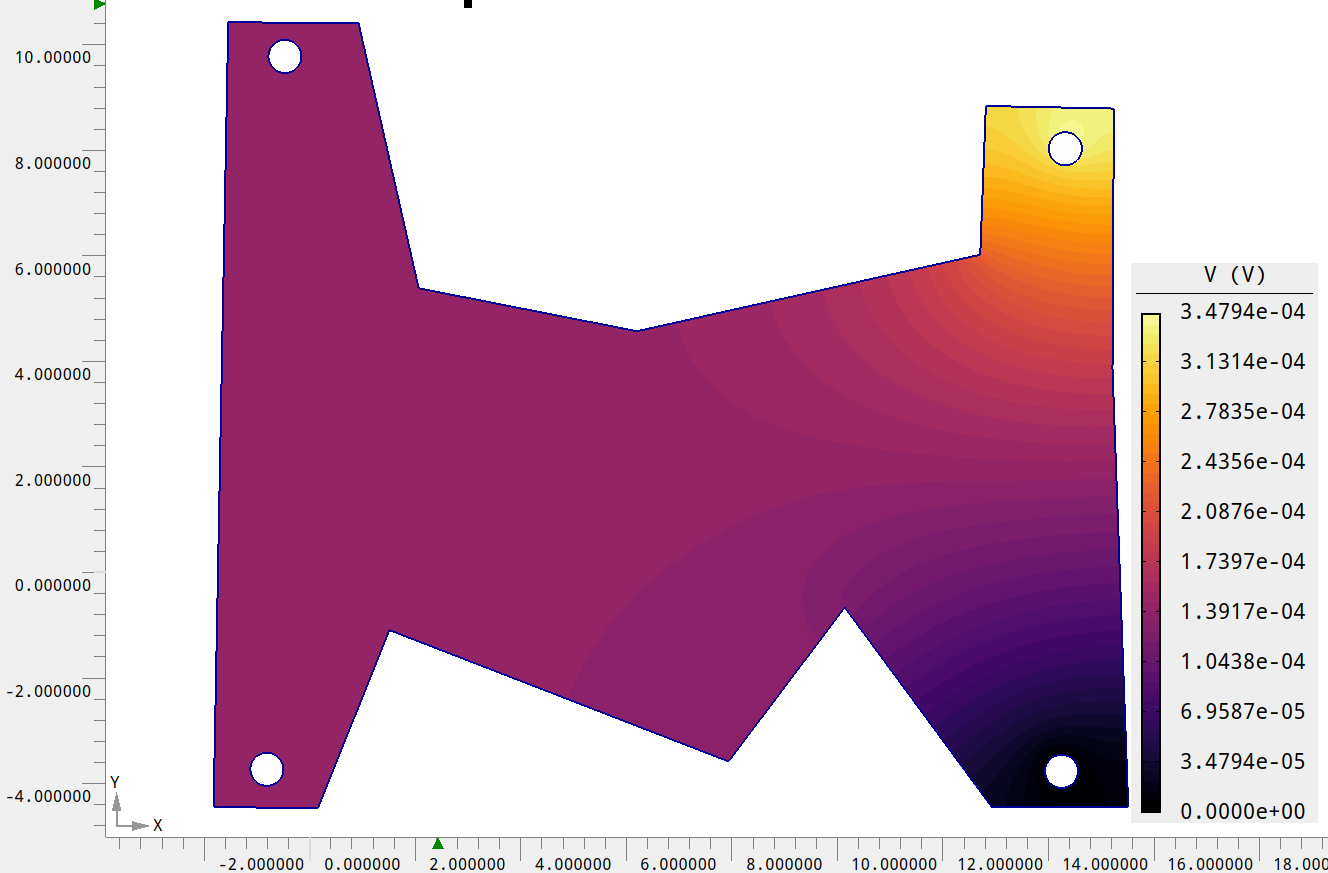
\includegraphics[width=1\linewidth]{Imagen Agros 1/Agros4.png}
	\end{center}  	
\end{minipage}

% Disposición 5
\subsection{Disposición 5}

\begin{table}[H]
    \centering
\begin{tabular}{cccc}
\toprule
$I$ [A] & $V$ [V] & $J_1$ [A/cm$^2$] & $J_2$ [A/cm$^2$] \\
\midrule
3.034 $\pm$ 0.032 & 0.8884 $\pm$ 0.0046 & 15.42 $\pm$ 0.16 & 12.37 $\pm$ 0.13 \\
\bottomrule
\end{tabular}
    \caption{Tabla de la valores para la disposición 5 $r_1=0.313$ y $r_2=0.390$ cm }
    \label{Tab:VIJ_mini_5}
\end{table}

\begin{table}[H]
    \centering
\begin{tabular}{c|cccc|ccc}
\toprule
\midrule
$V_+$ [mV] & \SI{2.191e-01}{} & \SI{2.190e-01}{} & \SI{2.193e-01}{} & \SI{2.191e-01}{} & $\overline{V}_+$ [$\mu$V] & $\overline{V}_-$ [$\mu$V] & $\Delta V_{\simu}$ [$\mu$V] \\
$V_-$ [mV] & \SI{0.3559}{} & \SI{0.3553}{} & \SI{0.3560}{} & \SI{0.3556}{} & \SI{355.70}{} $\pm$ 0.16 & \SI{219.12}{} $\pm$ 0.06 & \SI{136.57}{} $\pm$ 0.17 \\
\bottomrule
\end{tabular}
    \caption{Tabla de la valores para la disposición 5 de $V_+$ y $V_-$ con r=0.31 cm}
    \label{Tab:Vpn1_5}
\end{table}

\begin{table}[H]
    \centering
\begin{tabular}{c|cccc|ccc}
\toprule
\midrule
$V_+$ [mV] & \SI{3.507e-01}{} & \SI{3.500e-01}{} & \SI{3.509e-01}{} & \SI{3.504e-01}{} & $\overline{V}_+$ [$\mu$V] & $\overline{V}_-$ [$\mu$V] & $\Delta V_{\simu}$ [$\mu$V] \\
$V_-$ [mV] & \SI{0.2141}{} & \SI{0.2139}{} & \SI{0.2140}{} & \SI{0.2142}{} & \SI{214.05}{} $\pm$ 0.06 & \SI{350.50}{} $\pm$ 0.20 & \SI{136.45}{} $\pm$ 0.21 \\
\bottomrule
\end{tabular}
    \caption{Tabla de la valores para la disposición 5 de $V_+$ y $V_-$ con r=0.39 cm}
    \label{Tab:Vpn2_5}
\end{table}


\begin{minipage}[t]{0.45\linewidth} 
	\begin{center}
	\captionof{table}{Valores de $\sigma$ y $\rho$ para $r=0.313$ cm.}
	\vspace{0.5em}
	\begin{tabular}{ccc}
\toprule
$\sigma_{\exp}$ [S/cm] & $\rho_{\exp}$ [$\Omega$cm] \\
\midrule
\num{46119.428(247.737)} & \num{0.00002168(0.00000012)} \\
\bottomrule
\end{tabular}

	\vspace{1.2em}
	\captionof{table}{Valores de $\sigma$ y $\rho$ para $r=0.390$ cm.}
	\vspace{0.5em}
	\begin{tabular}{ccc}
\toprule
$\sigma_{\exp}$ [S/cm] & $\rho_{\exp}$ [$\Omega$cm] \\
\midrule
\num{46077.217(250.622)} & \num{0.00002170(0.00000012)} \\
\bottomrule
\end{tabular}

	\end{center}  
\end{minipage}
\hfill
\begin{minipage}[t]{0.45\linewidth}
	\begin{center}
	\captionof{figure}{Campo escalar para la disposición 5 con $r_1$.}
	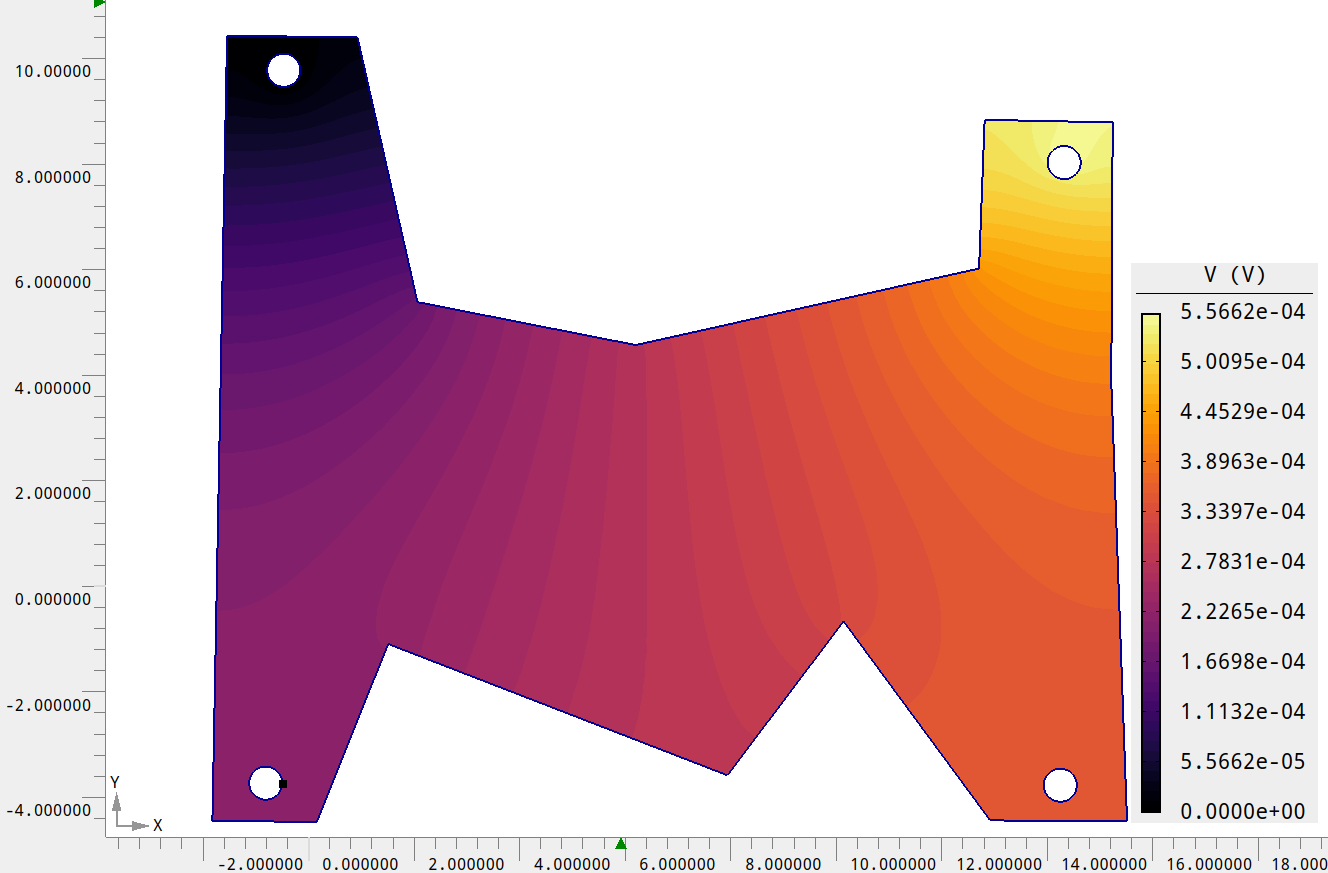
\includegraphics[width=1\linewidth]{Imagen Agros 1/Agros5.png}
	\end{center}  	
\end{minipage}


% Disposición 6v
\subsection{Disposición 6}


\begin{table}[H]
    \centering
\begin{tabular}{cccc}
\toprule
$I$ [A] & $V$ [V] & $J_1$ [A/cm$^2$] & $J_2$ [A/cm$^2$] \\
\midrule
3.070 $\pm$ 0.033 & 0.8969 $\pm$ 0.0047 & 15.60 $\pm$ 0.16 & 12.52 $\pm$ 0.13 \\
\bottomrule
\end{tabular}
    \caption{Tabla de la valores para la disposición 6 $r_1=0.313$ y $r_2=0.390$ cm }
    \label{Tab:VIJ_mini_6}
\end{table}

\begin{table}[H]
    \centering
\begin{tabular}{c|cccc|ccc}
\toprule
\midrule
$V_+$ [mV] & \SI{3.158e-01}{} & \SI{3.158e-01}{} & \SI{3.157e-01}{} & \SI{3.157e-01}{} & $\overline{V}_+$ [$\mu$V] & $\overline{V}_-$ [$\mu$V] & $\Delta V_{\simu}$ [$\mu$V] \\
$V_-$ [mV] & \SI{0.1775}{} & \SI{0.1776}{} & \SI{0.1776}{} & \SI{0.1776}{} & \SI{177.57}{} $\pm$ 0.03 & \SI{315.75}{} $\pm$ 0.03 & \SI{138.18}{} $\pm$ 0.04 \\
\bottomrule
\end{tabular}
    \caption{Tabla de la valores para la disposición 6 de $V_+$ y $V_-$ con r=0.31 cm}
    \label{Tab:Vpn1_6}
\end{table}

\begin{table}[H]
    \centering
\begin{tabular}{c|cccc|ccc}
\toprule
\midrule
$V_+$ [mV] & \SI{3.107e-01}{} & \SI{3.106e-01}{} & \SI{3.109e-01}{} & \SI{3.108e-01}{} & $\overline{V}_+$ [$\mu$V] & $\overline{V}_-$ [$\mu$V] & $\Delta V_{\simu}$ [$\mu$V] \\
$V_-$ [mV] & \SI{0.1727}{} & \SI{0.1726}{} & \SI{0.1727}{} & \SI{0.1726}{} & \SI{172.65}{} $\pm$ 0.03 & \SI{310.75}{} $\pm$ 0.06 & \SI{138.10}{} $\pm$ 0.07 \\
\bottomrule
\end{tabular}
    \caption{Tabla de la valores para la disposición 6 de $V_+$ y $V_-$ con r=0.39 cm}
    \label{Tab:Vpn2_6}
\end{table}


y el valor de la resistividad es: \\[1em]
\begin{minipage}[t]{0.45\linewidth} 
	\begin{center}
	\captionof{table}{Valores de $\sigma$ y $\rho$ para $r=0.313$ cm.}
	\vspace{0.5em}
	\begin{tabular}{ccc}
\toprule
$\sigma_{\exp}$ [S/cm] & $\rho_{\exp}$ [$\Omega$cm] \\
\midrule
\num{46217.527(241.731)} & \num{0.00002164(0.00000011)} \\
\bottomrule
\end{tabular}

	\vspace{1.2em}
	\captionof{table}{Valores de $\sigma$ y $\rho$ para $r=0.390$ cm.}
	\vspace{0.5em}
	\begin{tabular}{ccc}
\toprule
$\sigma_{\exp}$ [S/cm] & $\rho_{\exp}$ [$\Omega  \cdot$cm] \\
\midrule
\num{46192.441(242.419)} & \num{0.00002165(0.00000011)} \\
\bottomrule
\end{tabular}

	\end{center}  
\end{minipage}
\hfill
\begin{minipage}[t]{0.45\linewidth}
	\begin{center}
	\captionof{figure}{Campo escalar para la disposición 6 con $r_1$.}
	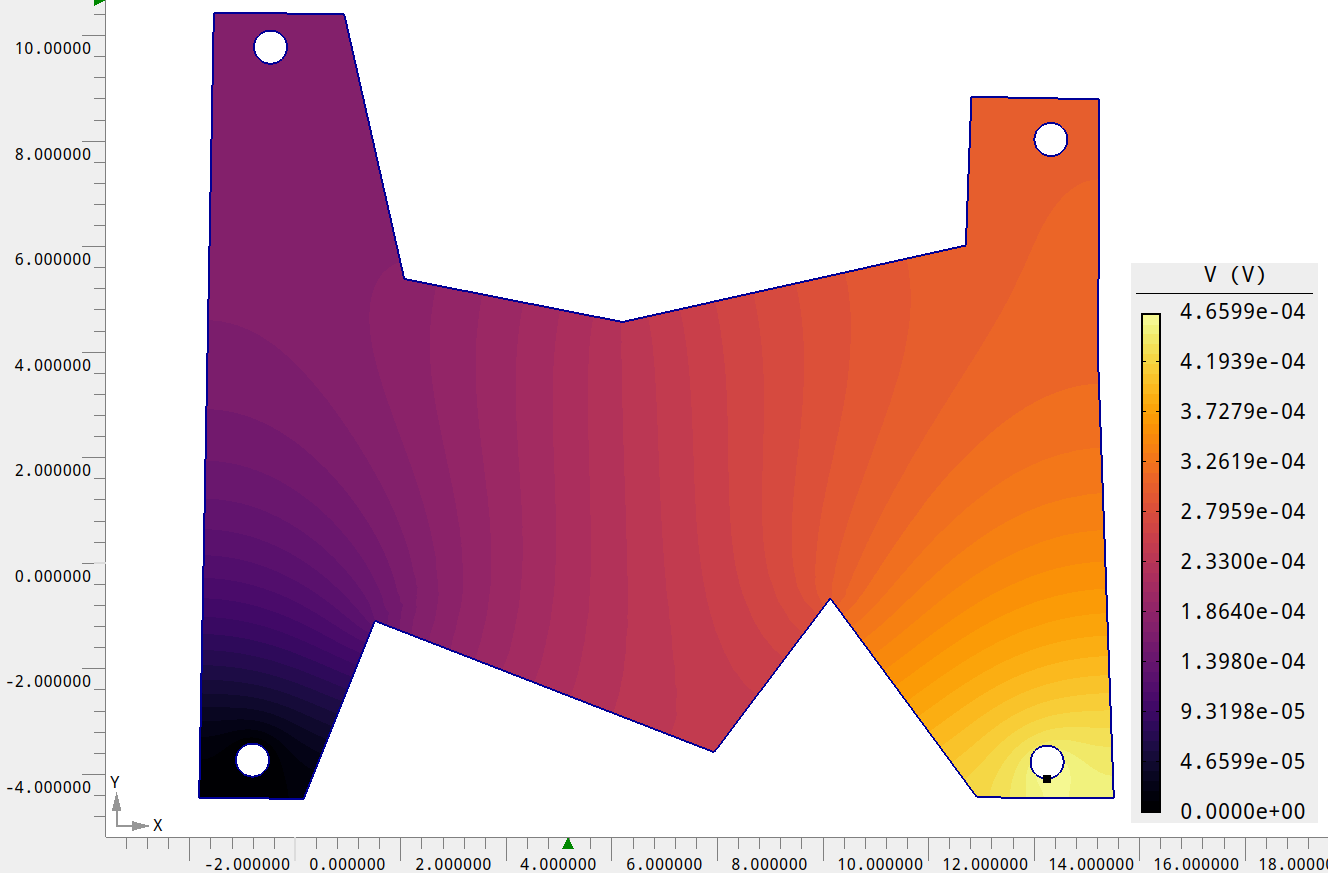
\includegraphics[width=1\linewidth]{Imagen Agros 1/Agros6.png}
	\end{center}  	
\end{minipage}



\subsection{Valores finales de la resistividad}

En esta sección obtendremos los valores de $\overline{\sigma_{\exp 1}}$ y $\overline{\sigma_{\exp 2}}$ que usaremos posteriormente en conclusiones para obtener un $\sigma_{\exp}$ final e identificar el metal. 

Para calcular los valores de la resistividad, tal y como hemos dicho, tenemos que realizar varias simulaciones en cada uno de los casos, obteniendo 6 valores de la resisitividad para cada radio. En principio $\sigma \neq \sigma (V)$, por lo que podríamos coger cualquier valor de $V$ para cada una de las simulaciones. En general nos hemos quedado siempre con el valor más grande de $V$ e $I$ porque minimiza el error dada por los voltímetros/amperímetros. \newpage

\begin{table}[H]
    \centering
\begin{tabular}{ccccc}
\toprule
 & $\sigma_{\exp}$ [S/cm] & $\rho_{\exp}$ [$\Omega$cm] \\
\midrule
Diposición 1 & \num{46428.984(250.320)} & \num{0.000021538(0.000000116)} \\
Diposición 2 & \num{46467.391(244.215)} & \num{0.000021520(0.000000113)} \\
Diposición 3 & \num{54545.455(5231.405)} & \num{0.000018333(0.000001758)} \\
Diposición 4 & \num{115384.615(18328.402)} & \num{0.000008667(0.000001377)} \\
Diposición 5 & \num{46119.428(247.737)} & \num{0.000021683(0.000000116)} \\
Diposición 6 & \num{46217.527(241.731)} & \num{0.000021637(0.000000113)} \\
\bottomrule
\end{tabular}
    \caption{Tabla de la valores para $r=0.31$ cm de $\sigma$ y $\rho $}
    \label{Tab:S1}
\end{table}

\begin{table}[H]
    \centering
\begin{tabular}{ccccc}
\toprule
 & $\sigma_{\exp}$ [S/cm] & $\rho_{\exp}$ [$\Omega \cdot$cm] \\
\midrule
Diposición 1 & \num{46420.323(252.117)} & \num{0.000021542(0.000000117)} \\
Diposición 2 & \num{46441.374(245.769)} & \num{0.000021533(0.000000114)} \\
Diposición 3 & \num{54545.455(5231.405)} & \num{0.000018333(0.000001758)} \\
Diposición 4 & \num{115384.615(18328.402)} & \num{0.000008667(0.000001377)} \\
Diposición 5 & \num{46077.217(250.622)} & \num{0.000021703(0.000000118)} \\
Diposición 6 & \num{46192.441(242.419)} & \num{0.000021649(0.000000114)} \\
\bottomrule
\end{tabular}
    \caption{Tabla de la valores para $r=0.39$ cm de $\sigma$ y $\rho $}
    \label{Tab:S2}
\end{table}


En las tablas \ref{Tab:S1} y \ref{Tab:S2} podemos ver los valores de $\sigma_{\exp}$ para cada disposición y radio elegido. Sin hacer un análisis estadístico profundo podemos ver directamente que los valores de las disposiciones 1,2,5 y 6 difieran mucho de las disposiciones 3 y 4, lo cual es de esperar (análisis más profundo de esta cuestión en el apartado \ref{Subsec:07_01}), mientras que las disposicioens 1,2,5 y 6 son muy parecidas entre sí. Lo que vamos a hacer a continuación es calcular una media ponderada \cite{Estadistica} de $\sigma_{\exp}$ ignorando las disposiciones 3 y 4, lo cual nos dará 2 valores de $\sigma_{\exp}$ que compararemos en \ref{Subsec:07_02}. 


Veamos pues los valores obtenidos finalmente (recordamos que son medias ponderadas obtenidas con las diposiciones 1,2,5 y 6), que son extremadamente parecidos entre sí. \\[1em]

\begin{table}[H]
    \centering
\begin{tabular}{ccccc}
\toprule
$\sigma_{\exp}$ [S/cm] & $\rho_{\exp}$ [$\Omega \cdot$cm] \\
\midrule
\num{46307.735(122.968)} & \num{0.000021595(0.000000057)} \\
\bottomrule
\end{tabular}
    \caption{Valor medio para $r=0.31$ cm de $\sigma$ y $\rho $}
    \label{Tab:S3}
\end{table}

\begin{table}[H]
    \centering
\begin{tabular}{ccccc}
\toprule
$\sigma_{\exp}$ [S/cm] & $\rho_{\exp}$ [$\Omega \cdot$cm] \\
\midrule
\num{46282.467(123.820)} & \num{0.000021606(0.000000058)} \\
\bottomrule
\end{tabular}
    \caption{Valor medio para $r=0.39$ cm de $\sigma$ y $\rho $}
    \label{Tab:S4}
\end{table}


\newpage

\section{Conclusiones}

En esta sección nos vamos a centrar en responder a todas las cuestiones que nos planteamos en los objetivos \ref{Sec:01}.

\subsection{¿Depende de $\sigma$ del a geometría?} \label{Subsec:07_01}

Tal y como nos deja ver las tablas \ref{Tab:S1} y \ref{Tab:S2}, los valores de las disposiciones que son cruzadas son muy parecidas entre sí (disposiciones 1 y 2) y con las disposiciones paralelas 3 y 4 (disposiciones 5 y 6), tanto para el radio $r=0.31$ cm y $r=0.39$ cm. De hecho podemos ver que todas las medidas cuadran en las incertidumbres de sus compañeras, lo cual es una medida de compatbilidad. El problema está, tal y como comentabamos más arriba, en las disposiciones 3 y 4 (paralelas 1 y 2). ¿Por qué puede ser esto?

La respuesta no es sencilla, aunque Manuel V. Ramallo ya nos dio un pequñeo comentario en el laboratorio de porque podría ocurrir esto. El problema con las diposiones paralelas presentadas es que la geometría es muy diferente, ya que es mucho mas parecido a una recta que a una placa dentada. Además al tener tan poca diferencia entre los valores de $\Delta V$ el error relativo es muchísimo más grande, con fuentes de incertidumbres más allá de las propidas del polímetro (como por ejemplo podría ser la luz incidente que modifique la conductividad localmente, diferencias de temperatura...). 

Sin embargo en aquellas que $\Delta V$ es ya de varios cientes de microvoltios este error se reduciría en comparación con los inherentes al polímetro. Sin hacer un análisis más detallado y extenso ($\chi^2$) creo que podemos afirmar que $\sigma$ no depende de la geometría salvo en aquellos casos que $\Delta V$ sea del orden de decenas microvoltios, en el que fuentes de incertidumbre, en principio desconcidos, pasan a un primer plano. 

\subsection{Valores de $\sigma_{\exp}$ e indentificación del metal.} \label{Subsec:07_02}

Una vez hemos obtenido los valores medios de $\sigma_{\exp}$ para ambas parametrizaciones, descartando las disposiciones 3 y 4 por razones evidentes (conductividades que no se corresponden con el material dado, por ejemplo para la disposición 3 tendríamos una conductividad del cobre) y viendo que los valores para ambas parametrizaciones de los terminales son compatibles, hacemos de nuevo una media ponderada obteniendo el siguiente valor de resisitivdad y condcutividad:

\begin{table}[H]
    \centering
\begin{tabular}{ccccc}
\toprule
$\sigma_{\exp}$ [S/cm] & $\rho_{\exp}$ [$\Omega \cdot$cm] \\
\midrule
\num{46295.188(87.251)} & \num{0.000021601(0.000000041)} \\
\bottomrule
\end{tabular}
    \caption{Valor medio definitvo de $\sigma$ y $\rho $}
    \label{Tab:S5}
\end{table}

que es el resultado final de nuestra prática. Ahora queda identificar nuestro metal. A priori parece que es Plomo (o una aleación con un alto contenido plomo). Según el \url{https://www.matweb.com/} $\rho_{\text{Pb}}=2.0643\times 10^{-5} \ \Omega\cdot$cm a 20$^oC$. Haciendo un análisis sencillo de chi cuadrado: 

\begin{equation}
	\chi^2 = \frac{\rho_{\exp}-\rho_{teo}}{u(\rho_{\exp})} 
\end{equation}
nos sale que el valor es incompatible con una confianza del 99.9\%. Sin embargo es normal, nosotros no realizamos las medidas a 20$^o$C (las medidas se hicieron nada más entrar al laboratorio por la mañana, por lo que la temperatura de la habitación estaría entorno a 12-15 $^o$C). ¿Podemos indentificar entonces el metal? Estadísticamente nos es imposible afirmar que tipo de material es. Para poder hacerlo tendríamos que contorlar rigurosamente las condiciones en las que medimos los valores y hacer que fueran constantes (luminosidad, tempeartura, humedad). 

Otras medidas que se nos ocurren que podríamos hacer para satisfacer la pregunta de qué metal es podría podría usar las disposiciones 3 y 4 teniendo en cuenta que se parece más a una disposición geométrica rectangular que a una dentada, con lo que midiendo $\Delta V$ entre los bornes en los que aplicamos la corriente y midiendo bien las distancias de la placa podríamos obtener $\rho$ facilmente. 


\appendix

\section{Tablas de datos} \label{Appendix:A}


\begin{table}[H]
    \centering
\begin{tabular}{cccc}
\toprule
$I$ [A] & $V$ [V] & $J_1$ [A/cm$^2$] & $J_2$ [A/cm$^2$] \\
\midrule
1.593 $\pm$ 0.018 & 0.4624 $\pm$ 0.0025 & 8.09 $\pm$ 0.08 & 6.50 $\pm$ 0.07 \\
1.984 $\pm$ 0.022 & 0.5748 $\pm$ 0.0031 & 10.08 $\pm$ 0.10 & 8.09 $\pm$ 0.08 \\
2.486 $\pm$ 0.027 & 0.7210 $\pm$ 0.0038 & 12.63 $\pm$ 0.13 & 10.14 $\pm$ 0.10 \\
2.988 $\pm$ 0.032 & 0.8660 $\pm$ 0.0045 & 15.18 $\pm$ 0.15 & 12.19 $\pm$ 0.12 \\
\bottomrule
\end{tabular}
    \caption{Tabla de la valores para la disposición 1 $r_1=0.313$ y $r_2= 0.390 $ cm }
    \label{Tab:VIJ_1}
\end{table}

\begin{table}[H]
    \centering
\begin{tabular}{cccc}
\toprule
$I$ [A] & $V$ [V] & $J_1$ [A/cm$^2$] & $J_2$ [A/cm$^2$] \\
\midrule
1.576 $\pm$ 0.018 & 0.4570 $\pm$ 0.0025 & 8.01 $\pm$ 0.08 & 6.43 $\pm$ 0.07 \\
1.979 $\pm$ 0.022 & 0.5733 $\pm$ 0.0031 & 10.06 $\pm$ 0.10 & 8.07 $\pm$ 0.08 \\
2.486 $\pm$ 0.027 & 0.7200 $\pm$ 0.0038 & 12.63 $\pm$ 0.13 & 10.14 $\pm$ 0.10 \\
2.986 $\pm$ 0.032 & 0.8648 $\pm$ 0.0045 & 15.17 $\pm$ 0.15 & 12.18 $\pm$ 0.12 \\
\bottomrule
\end{tabular}
    \caption{Tabla de la valores para la disposición 2 $r_1=0.313$ y $r_2= 0.390 $ cm }
    \label{Tab:VIJ_2}
\end{table}

\begin{table}[H]
    \centering
\begin{tabular}{cccc}
\toprule
$I$ [A] & $V$ [V] & $J_1$ [A/cm$^2$] & $J_2$ [A/cm$^2$] \\
\midrule
1.575 $\pm$ 0.018 & 0.0009 $\pm$ 0.0002 & 8.00 $\pm$ 0.08 & 6.42 $\pm$ 0.07 \\
2.020 $\pm$ 0.022 & 0.0014 $\pm$ 0.0002 & 10.26 $\pm$ 0.10 & 8.24 $\pm$ 0.08 \\
2.490 $\pm$ 0.027 & 0.0017 $\pm$ 0.0002 & 12.65 $\pm$ 0.13 & 10.15 $\pm$ 0.10 \\
3.051 $\pm$ 0.033 & 0.0022 $\pm$ 0.0002 & 15.50 $\pm$ 0.16 & 12.44 $\pm$ 0.13 \\
\bottomrule
\end{tabular}
    \caption{Tabla de la valores para la disposición 3 $r_1=0.313$ y $r_2= 0.390 $ cm }
    \label{Tab:VIJ_3}
\end{table}

\begin{table}[H]
    \centering
\begin{tabular}{cccc}
\toprule
$I$ [A] & $V$ [V] & $J_1$ [A/cm$^2$] & $J_2$ [A/cm$^2$] \\
\midrule
1.609 $\pm$ 0.018 & 0.0001 $\pm$ 0.0002 & 8.18 $\pm$ 0.08 & 6.56 $\pm$ 0.07 \\
1.970 $\pm$ 0.022 & 0.0002 $\pm$ 0.0002 & 10.01 $\pm$ 0.10 & 8.03 $\pm$ 0.08 \\
2.576 $\pm$ 0.028 & 0.0009 $\pm$ 0.0002 & 13.09 $\pm$ 0.13 & 10.51 $\pm$ 0.11 \\
2.963 $\pm$ 0.032 & 0.0013 $\pm$ 0.0002 & 15.06 $\pm$ 0.15 & 12.08 $\pm$ 0.12 \\
\bottomrule
\end{tabular}
    \caption{Tabla de la valores para la disposición 4 $r_1=0.313$ y $r_2= 0.390 $ cm }
    \label{Tab:VIJ_4}
\end{table}

\begin{table}[H]
    \centering
\begin{tabular}{cccc}
\toprule
$I$ [A] & $V$ [V] & $J_1$ [A/cm$^2$] & $J_2$ [A/cm$^2$] \\
\midrule
1.592 $\pm$ 0.018 & 0.4667 $\pm$ 0.0025 & 8.09 $\pm$ 0.08 & 6.49 $\pm$ 0.07 \\
2.024 $\pm$ 0.022 & 0.5915 $\pm$ 0.0032 & 10.29 $\pm$ 0.10 & 8.25 $\pm$ 0.08 \\
2.534 $\pm$ 0.027 & 0.7491 $\pm$ 0.0039 & 12.88 $\pm$ 0.13 & 10.33 $\pm$ 0.11 \\
3.034 $\pm$ 0.032 & 0.8884 $\pm$ 0.0046 & 15.42 $\pm$ 0.16 & 12.37 $\pm$ 0.13 \\
\bottomrule
\end{tabular}
    \caption{Tabla de la valores para la disposición 5 $r_1=0.313$ y $r_2= 0.390 $ cm }
    \label{Tab:VIJ_5}
\end{table}

\begin{table}[H]
    \centering
\begin{tabular}{cccc}
\toprule
$I$ [A] & $V$ [V] & $J_1$ [A/cm$^2$] & $J_2$ [A/cm$^2$] \\
\midrule
1.603 $\pm$ 0.018 & 0.4700 $\pm$ 0.0025 & 8.15 $\pm$ 0.08 & 6.54 $\pm$ 0.07 \\
2.020 $\pm$ 0.022 & 0.5908 $\pm$ 0.0032 & 10.26 $\pm$ 0.10 & 8.24 $\pm$ 0.08 \\
2.539 $\pm$ 0.027 & 0.7418 $\pm$ 0.0039 & 12.90 $\pm$ 0.13 & 10.35 $\pm$ 0.11 \\
3.070 $\pm$ 0.033 & 0.8969 $\pm$ 0.0047 & 15.60 $\pm$ 0.16 & 12.52 $\pm$ 0.13 \\
\bottomrule
\end{tabular}
    \caption{Tabla de la valores para la disposición 6 $r_1=0.313$ y $r_2= 0.390 $ cm }
    \label{Tab:VIJ_6}
\end{table}



	
\printbibliography

	



\end{document}